
          %------------------%
\chapter{~~Quotient manifolds}\label{\numb section 7}
          %------------------%


The roots of {\maniFEM} go back to a PhD thesis in 2002
% (or even earlier, to a Master thesis in 1997)
where finite elements on a torus were implemented in {\small\tt FORTRAN}.%
\footnote{See % C.~Barbarosie, Optimization of perforated domains through homogenization,
% Structural Optimization 14, 1997
C.~Barbarosie, Shape optimization of periodic structures,
Computers \& Structures 30, 2003}
The torus is meant as a mere quotient manifold between $ \mathbb{R}^2 $ and a group of
translations of $ \mathbb{R}^2 $ with two generators;
you may think of it as $ {\mathbb R}^2/{\mathbb Z}^2 $.
It should be stressed that this manifold is not the usual ``doughnut'' built in paragraph
\ref{\numb section 2.\numb parag 16}.
These two manifolds are homeomorphic (topologically equivalent) but they are not isometric,
that is, their geometry differ.
The quotient torus is a Riemann manifold with no curvature; it is locally Euclidian
(that is, locally isometric to open sets of $ \mathbb{R}^2 $); we may call it ``flat torus''.
It cannot be embedded in $ \mathbb{R}^3 $, much less be represented graphically.
An unfolded mesh in $ \mathbb{R}^2 $ can be represented graphically, where vertices and segments
from the torus are drawn more than once.

One of the goals of {\maniFEM} is to deal with meshes on quotient manifolds.
Different quotient operations can be used, with groups of translations of $ \mathbb{R}^2 $
but also with other groups of transformations.
In paragraphs \ref{\numb section 7.\numb parag 1} and \ref{\numb section 7.\numb parag 2}
we deal with a one-dimensional manifold, equivalent to a circle.
In paragraphs \ref{\numb section 7.\numb parag 3} and \ref{\numb section 7.\numb parag 16}
the quotient manifold is isometric to a cylinder.
In paragraphs \ref{\numb section 7.\numb parag 11} and \ref{\numb section 7.\numb parag 14}
we get a manifold homeomorphic (topologically equivalent) to a cylinder
if we eliminate the origin of the plane and we do not take into account that
rotations overlap.
In paragraphs \ref{\numb section 7.\numb parag 12} and \ref{\numb section 7.\numb parag 13}
the mesh contains the origin which is a singular point, thus the manifold reaches
the shape of a cone.
In paragraphs \ref{\numb section 7.\numb parag 4} -- \ref{\numb section 7.\numb parag 10},
\ref{\numb section 7.\numb parag 17} and \ref{\numb section 7.\numb parag 18}
the quotient manifold is homeomorphic to a torus.
The same holds for paragraph \ref{\numb section 7.\numb parag 15}
if we eliminate the origin of the plane and we do not take into account that
rotations overlap.
Note that in paragraphs \ref{\numb section 7.\numb parag 14} and
\ref{\numb section 7.\numb parag 15} the metric is not well-defined,
so the manifold we are dealing with is not a Riemannian manifold.

In paragraphs \ref{\numb section 7.\numb parag 3} -- \ref{\numb section 7.\numb parag 15},
a quotient manifold is declared and then a mesh is built directly on this manifold.
It is like holding a cylinder or a torus or a cone in your hand and drawing the mesh
directly on the cylinder or torus or cone.
In paragraphs \ref{\numb section 7.\numb parag 16} -- \ref{\numb section 7.\numb parag 18},
a mesh is built in the usual Euclidian plane and then is folded.
It is like drawing the mesh on a plane sheet of paper, then cutting the paper with a scissor
along the boundary of the mesh and then folding the resulting piece of paper
by glueing opposite faces.


          %--------------------------%
\section{~~A circle with no curvature}\label{\numb section 7.\numb parag 1}
          %--------------------------%

Here is the closed curve $ \mathbb{R}/{\mathbb Z} $.
We define it as a segment from {\small\tt A} to {\small\tt A}, with a specified
{\small\tt winding} number.

\begin{Verbatim}[commandchars=\\\{\},formatcom=\small\tt,frame=single,
   label=parag-\ref{\numb section 7.\numb parag 1}.cpp,rulecolor=\color{coment},
   baselinestretch=0.94,framesep=2mm                                            ]
   \cinza{// begin with the one-dimensional line}
   \verm{Manifold} \azul{RR} ( \textcolor{tag}{tag}::Euclid, \textcolor{tag}{tag}::of_dim, 1 );
   \verm{Function} \azul{x} = RR .build_coordinate_system ( \textcolor{tag}{tag}::Lagrange, \textcolor{tag}{tag}::of_degree, 1 );

   \cinza{// define an action on RR (a translation)}
   \verm{Manifold}::Action \azul{g} ( \textcolor{tag}{tag}::transforms, x, \textcolor{tag}{tag}::into, x+1. );
   \verm{Manifold} \azul{circle} = RR .quotient ( g );

   \cinza{// one vertex is enough to start the process}
   \verm{Cell} \azul{A} ( \textcolor{tag}{tag}::vertex );  x(A) = 0.02;
   \cinza{// with this vertex, we build a segment}
   \verm{Mesh} \azul{seg} ( \textcolor{tag}{tag}::segment, A .reverse(), A, \textcolor{tag}{tag}::divided_in, 10, \textcolor{tag}{tag}::winding, g );
\end{Verbatim}

We do not bother with the graphical representation of this one-dimensional mesh.

This mesh has 10 segments and 10 vertices. It has no boundary.
In contrast, if we mesh a segment in the usual Euclidian space $ \mathbb{R} $,
we get 10 segments and 11 vertices (and we get a boundary made of two vertices).

In an effort not to expose too many names in the {\small\tt namespace \verm{maniFEM}},
we have chosen to hide the class name {\small\tt Action} inside the namespace of
{\small\tt class \verm{Manifold}}.
See paragraph \ref{\numb section 11.\numb parag 1}.

Paragraph \ref{\numb section 11.\numb parag 2} explains the coloring conventions observed
in this manual for {\tt C++} code.
Paragraph \ref{\numb section 11.\numb parag 3} gives details about
{\small\tt\textcolor{tag}{tag}}s.


          %---------------%
\section{~~A curved circle}\label{\numb section 7.\numb parag 2}
          %---------------%

We are now in a position to resume the example in paragraph \ref{\numb section 2.\numb parag 15},
this time in a less cumbersome manner.

\begin{Verbatim}[commandchars=\\\{\},formatcom=\small\tt,frame=single,
   label=parag-\ref{\numb section 7.\numb parag 2}.cpp,rulecolor=\color{coment},
   baselinestretch=0.94,framesep=2mm                                            ]
   \verm{Manifold} \azul{RR} ( \textcolor{tag}{tag}::Euclid, \textcolor{tag}{tag}::of_dim, 1 );
   \verm{Function} \azul{theta} = RR .build_coordinate_system ( \textcolor{tag}{tag}::Lagrange, \textcolor{tag}{tag}::of_degree, 1 );

   const double \azul{pi} = 3.1415926536;
   \verm{Manifold}::Action \azul{g} ( \textcolor{tag}{tag}::transforms, theta, \textcolor{tag}{tag}::into, theta + 2*pi );
   \verm{Manifold} \azul{circle} = RR .quotient ( g );

   \verm{Cell} \azul{A} ( \textcolor{tag}{tag}::vertex );  theta ( A ) = 0.;
   \verm{Mesh} \azul{loop} ( \textcolor{tag}{tag}::segment, A.reverse(), A, \textcolor{tag}{tag}::divided_in, 20, \textcolor{tag}{tag}::winding, g );

   \cinza{// define new coordinates x and y as arithmetic expressions of theta}
   \verm{Function} \azul{x} = \verm{cos} (theta), \azul{y} = \verm{sin} (theta);

   \cinza{// forget about theta; in future statements, x and y will be used}
   circle .set_coordinates ( x && y );
   loop .export_msh (\verde{"circle.msh"});
\end{Verbatim}

In {\tt gmsh}, you must select {\small\tt Tools} $\to$ {\small\tt Options} $\to$
{\small\tt Mesh} $\to$ {\small\tt 1D Elements} in order to see this mesh.


          %----------%
\section{~~A cylinder}\label{\numb section 7.\numb parag 3}
          %----------%

Here is how to build a (part of a) cylinder in $ \mathbb{R}^3 $ :

\begin{Verbatim}[commandchars=\\\{\},formatcom=\small\tt,frame=single,
   label=parag-\ref{\numb section 7.\numb parag 3}.cpp,rulecolor=\color{coment},
   baselinestretch=0.94,framesep=2mm                                            ]
   \verm{Manifold} \azul{RR2} ( \textcolor{tag}{tag}::Euclid, \textcolor{tag}{tag}::of_dim, 2 );
   \verm{Function} \azul{theta_z} =
      RR2 .build_coordinate_system ( \textcolor{tag}{tag}::Lagrange, \textcolor{tag}{tag}::of_degree, 1 );
   \verm{Function} \azul{theta} = theta_z [0], \azul{z} = theta_z [1];

   const double \azul{pi} = 3.1415926536;
   \verm{Manifold}::Action \azul{g} ( \textcolor{tag}{tag}::transforms, theta_z, \textcolor{tag}{tag}::into, (theta+2*pi) && z );
   \verm{Manifold} \azul{cylinder_manif} = RR2 .quotient ( g );

   \verm{Cell} \azul{A} ( \textcolor{tag}{tag}::vertex );  theta (A) = 0.;  z (A) = -1.;
   \verm{Cell} \azul{B} ( \textcolor{tag}{tag}::vertex );  theta (B) = 0.;  z (B) =  1.;

   \verm{Mesh} \azul{AA} ( \textcolor{tag}{tag}::segment, A .reverse(), A, \textcolor{tag}{tag}::divided_in, 20, \textcolor{tag}{tag}::winding,  g );
   \verm{Mesh} \azul{AB} ( \textcolor{tag}{tag}::segment, A .reverse(), B, \textcolor{tag}{tag}::divided_in, 15 );  \cinza{// no winding}
   \verm{Mesh} \azul{BB} ( \textcolor{tag}{tag}::segment, B .reverse(), B, \textcolor{tag}{tag}::divided_in, 20, \textcolor{tag}{tag}::winding, -g );

   \verm{Mesh} \azul{cylinder} ( \textcolor{tag}{tag}::rectangle, AA, AB, BB, AB .reverse(), \textcolor{tag}{tag}::winding );
   \cinza{// define new coordinates x and y as arithmetic expressions of theta}
   \verm{Function} \azul{x} = \verm{cos}(theta), \azul{y} = \verm{sin}(theta);

   \cinza{// forget about theta; in future statements, x, y and z will be used}
   cylinder_manif .set_coordinates ( x && y & z );
   cylinder .export_msh (\verde{"cylinder.msh"});
\end{Verbatim}

The {\small\tt\textcolor{tag}{tag}::winding} in the constructor {\small\tt\verm{Mesh}
\azul{cylinder}} provides no specific information, it just warns {\maniFEM} that
we are on a quotient manifold and that it must take winding numbers into account.
Specific information about these winding numbers is included in the three segments
{\small\tt AA}, {\small\tt AB} and {\small\tt BB}.

Note the additive syntax used to represent composition of actions.
The expression {\small\tt -g} stands for the inverse of {\small\tt g}.
In subsequent paragraphs, we shall encounter expressions like
{\small\tt g2} {\small\tt -} {\small\tt g1} which stands for the composition between
{\small\tt g2} and the inverse of {\small\tt g1} (we assume the action group is commutative).

Some people may prefer a multiplicative notation like {\small\tt pow} {\small\tt (} {\small\tt g,}
{\small\tt -1} {\small\tt )} or {\small\tt g2} {\small\tt /} {\small\tt g1};
we have chosen the additive syntax because it allows for expressions like {\small\tt -5*g2}
{\small\tt +} {\small\tt 3*g1} which become somewhat cumbersome if we use
the multiplicative notation.
Besides that, the composition of translations corresponds to the sum of the vectors
defining the translations.


          %------------%
\section{~~A flat torus}\label{\numb section 7.\numb parag 4}
          %------------%

Here is the classical example of $ \mathbb{R}^2/{\mathbb Z}^2 $.

\begin{Verbatim}[commandchars=\\\{\},formatcom=\small\tt,frame=single,
   label=parag-\ref{\numb section 7.\numb parag 4}.cpp,rulecolor=\color{coment},
   baselinestretch=0.94,framesep=2mm                                            ]
   \cinza{// begin with the usual two-dimensional space}
   \verm{Manifold} \azul{RR2} ( \textcolor{tag}{tag}::Euclid, \textcolor{tag}{tag}::of_dim, 2 );
   \verm{Function} \azul{xy} = RR2 .build_coordinate_system ( \textcolor{tag}{tag}::Lagrange, \textcolor{tag}{tag}::of_degree, 1 );
   \verm{Function} \azul{x} = xy [0], \azul{y} = xy [1];

   \cinza{// define two actions on RR2 (translations)}
   \verm{Manifold}::Action \azul{g_horiz} ( \textcolor{tag}{tag}::transforms, xy, \textcolor{tag}{tag}::into, (x+1.) && y ),
                    \azul{g_vert}  ( \textcolor{tag}{tag}::transforms, xy, \textcolor{tag}{tag}::into, x && (y+1.) );
   \verm{Manifold} \azul{torus_manif} = RR2 .quotient ( g_horiz, g_vert );

   \cinza{// one vertex is enough to start the process}
   \verm{Cell} \azul{A} ( \textcolor{tag}{tag}::vertex );  x (A) = 0.02;  y (A) = 0.02;
   \cinza{// with this vertex, we build two segments}
   \verm{Mesh} \azul{seg_horiz} ( \textcolor{tag}{tag}::segment, A .reverse(), A,
                    \textcolor{tag}{tag}::divided_in, 10, \textcolor{tag}{tag}::winding, g_horiz );
   \verm{Mesh} \azul{seg_vert}  ( \textcolor{tag}{tag}::segment, A .reverse(), A,
                    \textcolor{tag}{tag}::divided_in, 10, \textcolor{tag}{tag}::winding, g_vert  );
   \cinza{// and a rectangle}
   \verm{Mesh} \azul{torus} ( \textcolor{tag}{tag}::rectangle, seg_horiz, seg_vert,
                seg_horiz .reverse(), seg_vert .reverse(), \textcolor{tag}{tag}::winding );

   \cinza{// it would be meaningless to export 'torus' as a msh file}
   \cinza{// we can however draw an unfolded mesh :}
   torus .draw_ps (\verde{"torus.eps"}, \textcolor{tag}{tag}::unfold,
                    \textcolor{tag}{tag}::over_region, -0.5 < x < 1.5, -0.2 < y < 1.2 );
\end{Verbatim}

The {\small\tt\textcolor{tag}{tag}::winding} in the constructor {\small\tt\verm{Mesh}}
{\small\tt\azul{torus}} provides no specific information, it just warns {\maniFEM} that
we are on a quotient manifold and that it must take winding numbers into account.
Specific information about the winding numbers is included in the two segments
{\small\tt seg\_\,horiz} and {\small\tt seg\_\,vert}.

This quotient torus is a Riemann manifold with no curvature; it is locally Euclidian
(that is, locally isometric to open sets of $ \mathbb{R}^2 $); we may call it ``flat torus''.
It cannot be embedded in $ \mathbb{R}^3 $, much less be represented graphically.
An unfolded mesh in $ \mathbb{R}^2 $ can be represented graphically,
as in figure \ref{\numb section 7.\numb fig 1}, where vertices and segments from the torus
are drawn more than once.

The mesh {\small\tt torus} has 100 squares, 200 segments and 100 vertices.
It has no boundary, it is closed in itself, it covers entirely $ \mathbb{R}^2/{\mathbb Z}^2 $
which is a compact manifold with no boundary.
In contrast, if we mesh the square $ [0,1]^2 $ in the usual Euclidian plane
we get a mesh with 100 squares, 220 segments and 121 vertices (and of course we get a boundary).

In figure \ref{\numb section 7.\numb fig 1} we have added a shadow representing
the periodicity cell $ [0,1]^2 $.
This gives a hint about the repeated structure of the the unfolded mesh.
We see that, for instance, the vertex {\small\tt A} shows up four times.
Each segment originating from {\small\tt A} is also drawn four times.
Other vertices and segments are drawn only twice, or only once.
These numbers depend on the position of the vertex or segment and on the shape and size
of the viewing window.

\begin{figure}[ht] \centering
  \psfrag{A}{\small\tt\textcolor{textindraw}{A}}
  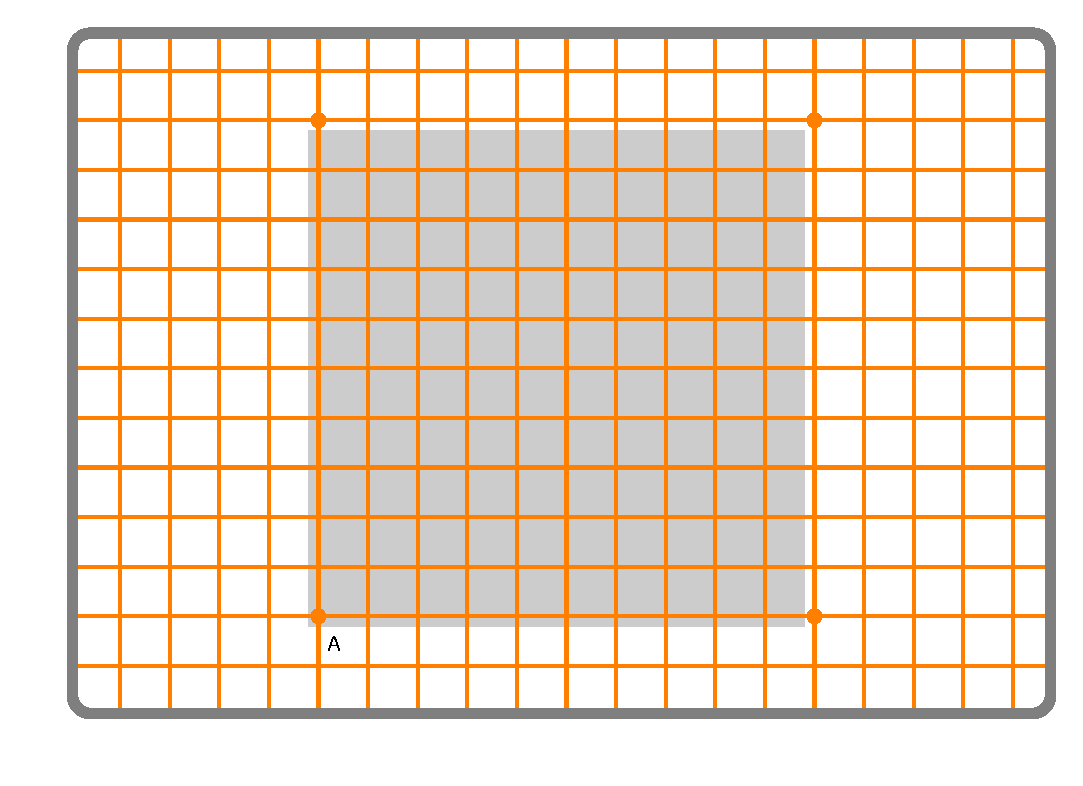
\includegraphics[width=76mm]{flat-torus-1.eps}
  \caption{A flat torus}
  \label{\numb section 7.\numb fig 1}
\end{figure}

Figure \ref{\numb section 7.\numb fig 1} is rather dull because the mesh is very regular.
In paragraphs \ref{\numb section 7.\numb parag 6} -- \ref{\numb section 7.\numb parag 9}
we introduce an inhomogeneity (a small hole) in the mesh in order to turn the repetitive pattern
more visible.

The comment at the end of the above code excerpt says that it makes no sense to export
{\small\tt torus} in {\small\tt msh} format.
We can however build an unfolded mesh which lives in {\small\tt RR2} rather than in
{\small\tt quotient\_\,manifold}, and this unfolded mesh accepts all methods of two-dimensional
meshes, including {\small\tt export\_\,msh}.
Paragraph \ref{\numb section 7.\numb parag 6} shows an example.

If you feel uncomfortable with this minimalist approach (of defining a square with only one
vertex), you may think in terms of four squares instead :

\begin{Verbatim}[commandchars=\\\{\},formatcom=\small\tt,
   baselinestretch=0.94,framesep=2mm                      ]
   \verm{Cell} \azul{A} ( \textcolor{tag}{tag}::vertex );  x (A) = 0. ;  y (A) = 0. ;
   \verm{Cell} \azul{B} ( \textcolor{tag}{tag}::vertex );  x (B) = 0.5;  y (B) = 0. ;
   \verm{Cell} \azul{C} ( \textcolor{tag}{tag}::vertex );  x (C) = 0.5;  y (C) = 0.5;
   \verm{Cell} \azul{D} ( \textcolor{tag}{tag}::vertex );  x (D) = 0. ;  y (D) = 0.5;
   \verm{Mesh} \azul{AB} ( \textcolor{tag}{tag}::segment, A.reverse(), B, \textcolor{tag}{tag}::divided_in, 5 ),
        \azul{BC} ( \textcolor{tag}{tag}::segment, B .reverse(), C, \textcolor{tag}{tag}::divided_in, 5 ),
        \azul{CD} ( \textcolor{tag}{tag}::segment, C .reverse(), D, \textcolor{tag}{tag}::divided_in, 5 ),
        \azul{DA} ( \textcolor{tag}{tag}::segment, D .reverse(), A, \textcolor{tag}{tag}::divided_in, 5 ),
        \azul{BA1} ( \textcolor{tag}{tag}::segment, B .reverse(), A, \textcolor{tag}{tag}::divided_in, 5, \textcolor{tag}{tag}::winding, g_horiz ),
        \azul{CD1} ( \textcolor{tag}{tag}::segment, C .reverse(), D, \textcolor{tag}{tag}::divided_in, 5, \textcolor{tag}{tag}::winding, g_horiz ),
        \azul{CB2} ( \textcolor{tag}{tag}::segment, C .reverse(), B, \textcolor{tag}{tag}::divided_in, 5, \textcolor{tag}{tag}::winding, g_vert ),
        \azul{DA2} ( \textcolor{tag}{tag}::segment, D .reverse(), A, \textcolor{tag}{tag}::divided_in, 5, \textcolor{tag}{tag}::winding, g_vert );

   \verm{Mesh} \azul{sq1} ( \textcolor{tag}{tag}::rectangle, AB, BC, CD, DA ),
        \azul{sq2} ( \textcolor{tag}{tag}::rectangle, BA1, DA .reverse(), CD1 .reverse(),
                              BC .reverse(), \textcolor{tag}{tag}::winding ),
        \azul{sq3} ( \textcolor{tag}{tag}::rectangle, DA2 .reverse(), CD .reverse(), CB2,
                              AB .reverse(), \textcolor{tag}{tag}::winding ),
        \azul{sq4} ( \textcolor{tag}{tag}::rectangle, CD1, DA2, BA1 .reverse(), CB2 .reverse(), \textcolor{tag}{tag}::winding );
	
   \verm{Mesh} \azul{torus} ( \textcolor{tag}{tag}::join, sq1, sq2, sq3, sq4 );
\end{Verbatim}


          %--------------%
\section{~~A curved torus}\label{\numb section 7.\numb parag 5}
          %--------------%

We are now in a position to resume the example in paragraph \ref{\numb section 2.\numb parag 16},
this time by using the quotient manifold $ \mathbb{R}^2/{\mathbb Z}^2 $ introduced in paragraph
\ref{\numb section 7.\numb parag 4}.

\begin{Verbatim}[commandchars=\\\{\},formatcom=\small\tt,frame=single,
   label=parag-\ref{\numb section 7.\numb parag 5}.cpp,rulecolor=\color{coment},
   baselinestretch=0.94,framesep=2mm                                            ]
   \verm{Manifold} \azul{RR2} ( \textcolor{tag}{tag}::Euclid, \textcolor{tag}{tag}::of_dim, 2 );
   \verm{Function} \azul{ab} = RR2 .build_coordinate_system ( \textcolor{tag}{tag}::Lagrange, \textcolor{tag}{tag}::of_degree, 1 );
   \verm{Function} \azul{alpha} = ab [0], \azul{beta} = ab [1];

   const double \azul{pi} = 3.1415926536;
   \verm{Manifold}::Action \azul{g1} ( \textcolor{tag}{tag}::transforms, ab, \textcolor{tag}{tag}::into, (alpha+2.*pi) && beta );
   \verm{Manifold}::Action \azul{g2} ( \textcolor{tag}{tag}::transforms, ab, \textcolor{tag}{tag}::into, alpha && (beta+2.*pi) );
   \verm{Manifold} \azul{torus_manif} = RR2 .quotient ( g1, g2 );

   \verm{Cell} \azul{A} ( \textcolor{tag}{tag}::vertex );  alpha (A) = 0.;  beta (A) = 0.;
   \verm{Mesh} \azul{seg_horiz} ( \textcolor{tag}{tag}::segment, A .reverse(), A,
                    \textcolor{tag}{tag}::divided_in, 40, \textcolor{tag}{tag}::winding, g1 );
   \verm{Mesh} \azul{seg_vert}  ( \textcolor{tag}{tag}::segment, A .reverse(), A,
                    \textcolor{tag}{tag}::divided_in, 20, \textcolor{tag}{tag}::winding, g2 );
   \verm{Mesh} \azul{torus} ( \textcolor{tag}{tag}::rectangle, seg_horiz, seg_vert,
                seg_horiz .reverse(), seg_vert .reverse(), \textcolor{tag}{tag}::winding );

   \cinza{// parametrize the doughnut}
   const double \azul{big_radius} = 3., \azul{small_radius} = 1.;
   \cinza{// define x, y and z as functions of alpha and beta}
   \verm{Function} \azul{x} = ( big_radius + small_radius*\verm{cos}(beta) ) * \verm{cos}(alpha),
            \azul{y} = ( big_radius + small_radius*\verm{cos}(beta) ) * \verm{sin}(alpha),
            \azul{z} = small_radius*\verm{sin}(beta);

   \cinza{// forget about alpha and beta :}
   torus_manif .set_coordinates ( x && y && z );
   \cinza{// in future statements (e.g. for graphical representation)}
   \cinza{// x, y and z will be used, not alpha nor beta :}
   torus .export_msh (\verde{"torus.msh"});
\end{Verbatim}


          %------------------------%
\section{~~A flat torus with a hole}\label{\numb section 7.\numb parag 6}
          %------------------------%

In this paragraph, we perforate the flat torus.
This small inhomogeneity makes the drawing more meaningful.
We also change the shape of the viewing window, just for the fun of it.

We stress that this mesh has only one hole; figure \ref{\numb section 7.\numb fig 2}
shows several images of the same hole, due to the unfolding.

\begin{Verbatim}[commandchars=\\\{\},formatcom=\small\tt,frame=single,
   label=parag-\ref{\numb section 7.\numb parag 6}.cpp,rulecolor=\color{coment},
   baselinestretch=0.94,framesep=2mm                                            ]
   std::vector < \verm{Cell} > \azul{vec};

   \verm{Mesh}::Iterator \azul{it} = torus .iterator
      ( \textcolor{tag}{tag}::over_cells, \textcolor{tag}{tag}::of_dim, 2, \textcolor{tag}{tag}::around, A );
   for ( it .reset(); it .in_range(); it++ ) vec .push_back ( *it );
   std::vector < \verm{Cell} > ::iterator \azul{itv};
   for ( itv = vec .begin(); itv != vec .end(); itv++ )
   \{  \verm{Cell} \azul{sq} = *itv;  sq .remove_from_mesh ( torus );  \}

   \cinza{// we can draw an unfolded mesh :}
   torus .draw_ps (\verde{"torus.eps"}, \textcolor{tag}{tag}::unfold,
                    \textcolor{tag}{tag}::over_region, x*x + 2.*y*y < 3.5 );

   \cinza{// or we can build a new, unfolded mesh and subsequently export as msh file}
   \verm{Mesh} \azul{unfolded} = torus .unfold ( \textcolor{tag}{tag}::over_region, x*x + 2.*y*y < 3.5 );
   unfolded .export_msh ("torus.msh");
\end{Verbatim}

\begin{figure}[ht] \centering
  \psfrag{A}{\small\tt\textcolor{textindraw}{A}}
  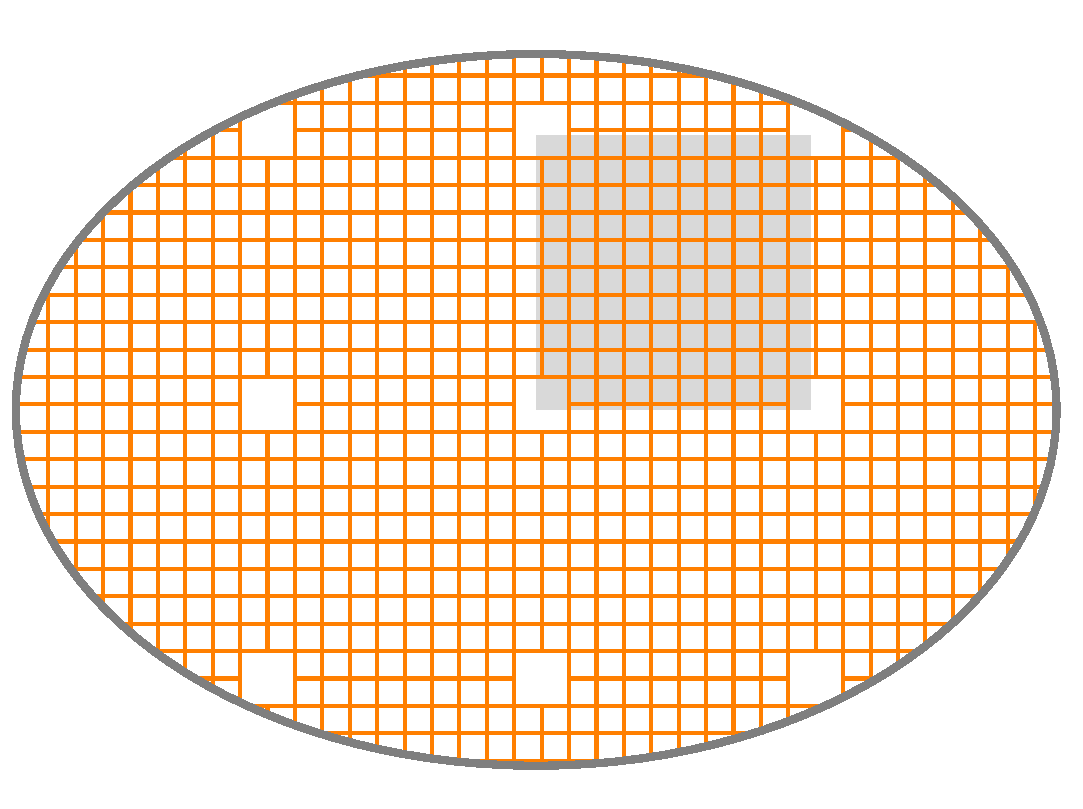
\includegraphics[width=92mm]{flat-torus-2.eps}
  \caption{A flat torus with a hole}
  \label{\numb section 7.\numb fig 2}
\end{figure}

Paragraph \ref{\numb section 9.\numb parag 8} describes iterators around a vertex.

As explained in paragraph \ref{\numb section 10.\numb parag 3}, it is not safe to
modify a mesh while iterating over its cells.
This is why we use a vector of cells (in paragraph \ref{\numb section 10.\numb parag 3}
a list of cells is used, both are OK).

          %-----------------%
\section{~~A skew flat torus}\label{\numb section 7.\numb parag 7}
          %-----------------%

We can build a skew torus by simply choosing other actions on {\small\tt RR2}.

\begin{figure}[ht] \centering
  \psfrag{A}{\small\tt\textcolor{textindraw}{A}}
  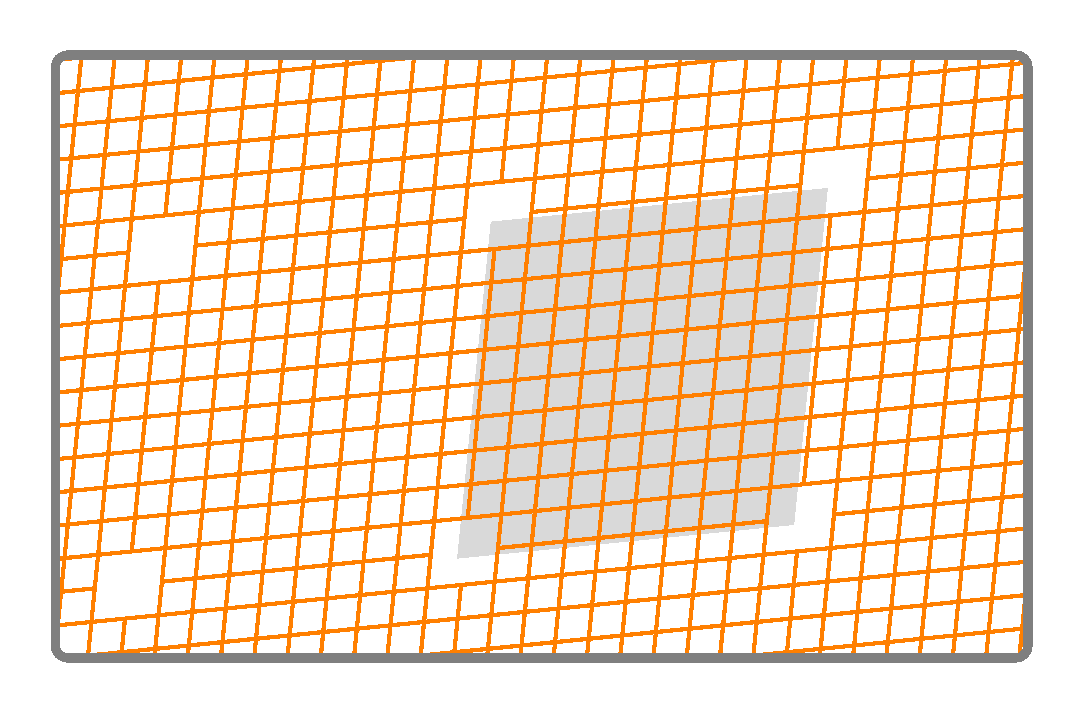
\includegraphics[width=76mm]{flat-torus-3.eps}
  \caption{A skew flat torus}
  \label{\numb section 7.\numb fig 3}
\end{figure}

\begin{Verbatim}[commandchars=\\\{\},formatcom=\small\tt,frame=single,
   label=parag-\ref{\numb section 7.\numb parag 7}.cpp,rulecolor=\color{coment},
   baselinestretch=0.94,framesep=2mm                                            ]
   \verm{Manifold}::Action \azul{g1} ( \textcolor{tag}{tag}::transforms, xy, \textcolor{tag}{tag}::into, (x+1.) && (y+0.1) );
   \verm{Manifold}::Action \azul{g2} ( \textcolor{tag}{tag}::transforms, xy, \textcolor{tag}{tag}::into, (x+0.1) && (y+1.) );
   \verm{Manifold} \azul{torus_manif} = RR2 .quotient ( g1, g2 );
\end{Verbatim}

Again, we have added a shadow representing the periodicity cell, this time a parallelogram.


          %-------------------%
\section{~~A skew torus, again}\label{\numb section 7.\numb parag 8}
          %-------------------%

Here is a different example of a skew torus, this time meshed with square cells
rather than skew parallelograms.

\begin{figure}[ht] \centering
  \psfrag{A}{\small\tt\textcolor{textindraw}{A}}
  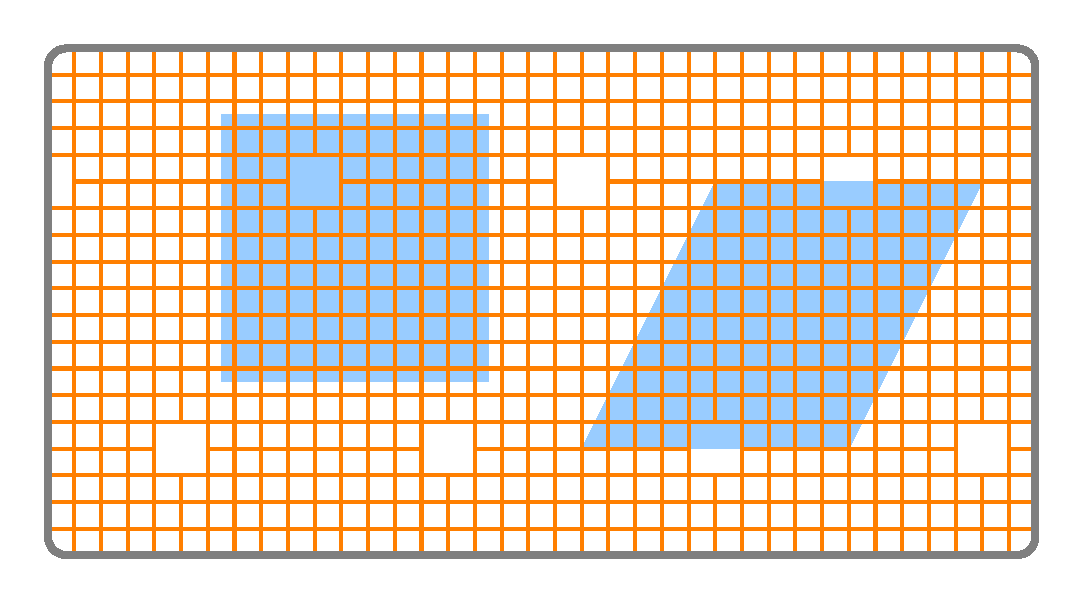
\includegraphics[width=92mm]{flat-torus-4.eps}
  \caption{A different torus}
  \label{\numb section 7.\numb fig 4}
\end{figure}

\begin{Verbatim}[commandchars=\\\{\},formatcom=\small\tt,frame=single,
   label=parag-\ref{\numb section 7.\numb parag 8}.cpp,rulecolor=\color{coment},
   baselinestretch=0.94,framesep=2mm                                            ]
   \verm{Manifold}::Action \azul{g1} ( \textcolor{tag}{tag}::transforms, xy, \textcolor{tag}{tag}::into, (x+1.) && y ),
                    \azul{g2} ( \textcolor{tag}{tag}::transforms, xy, \textcolor{tag}{tag}::into, (x+0.5) && (y+1.) );
   \verm{Manifold} \azul{torus_manif} = RR2 .quotient ( g1, g2 );
   \verm{Cell} \azul{A} ( \textcolor{tag}{tag}::vertex );  x (A) = 0. ;  y (A) = 0.;
   \verm{Cell} \azul{B} ( \textcolor{tag}{tag}::vertex );  x (B) = 0.5;  y (B) = 0.;
   \verm{Mesh} \azul{AB} ( \textcolor{tag}{tag}::segment, A .reverse(), B, \textcolor{tag}{tag}::divided_in, 5 );
   \verm{Mesh} \azul{BA_horiz} ( \textcolor{tag}{tag}::segment, B .reverse(), A, \textcolor{tag}{tag}::divided_in, 5,
                  \textcolor{tag}{tag}::winding, g1                                  );
   \verm{Mesh} \azul{BA_vert} ( \textcolor{tag}{tag}::segment, B .reverse(), A, \textcolor{tag}{tag}::divided_in, 10,
                  \textcolor{tag}{tag}::winding, g2                                  );
   \verm{Mesh} \azul{AB_vert}
      ( \textcolor{tag}{tag}::segment, A .reverse(), B, \textcolor{tag}{tag}::divided_in, 10, \textcolor{tag}{tag}::winding, g2 - g1 );
   \verm{Mesh} \azul{sq1} ( \textcolor{tag}{tag}::rectangle, AB, BA_vert, BA_horiz .reverse(), AB_vert .reverse(),
              \textcolor{tag}{tag}::winding                                                        );
   \verm{Mesh} \azul{sq2} ( \textcolor{tag}{tag}::rectangle, BA_vert .reverse(), BA_horiz, AB_vert, AB .reverse(),
              \textcolor{tag}{tag}::winding                                                        );
   \verm{Mesh} \azul{torus} ( \textcolor{tag}{tag}::join, sq1, sq2 );
\end{Verbatim}

Note the additive syntax for composing actions; comments in paragraph
\ref{\numb section 7.\numb parag 3} apply.

In figure \ref{\numb section 7.\numb fig 4} we have drawn two shadows.
The skew parallelogram can be called ``periodicity cell'';
we call the other one ``representative domain''.

\begin{figure}[ht] \centering
  \psfrag{A}{\small\tt\textcolor{textindraw}{A}}
  \psfrag{B}{\small\tt\textcolor{textindraw}{B}}
  \psfrag{AB}{\small\tt\textcolor{textindraw}{AB}}
  \psfrag{BAh}{\small\tt\textcolor{textindraw}{BA\_\,horiz}}
  \psfrag{ABv}{\small\tt\textcolor{textindraw}{AB\_\,vert}}
  \psfrag{BAv}{\small\tt\textcolor{textindraw}{BA\_\,vert}}
  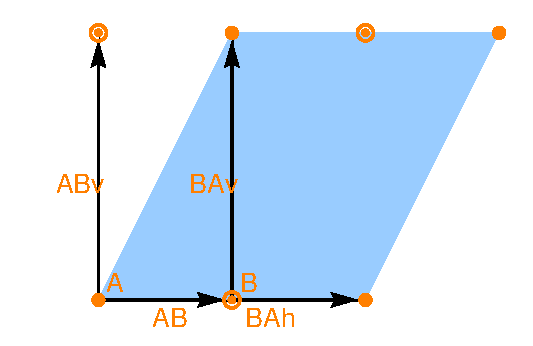
\includegraphics[width=60mm]{torus-sketch.eps}
  \caption{Segment meshes used for building the torus}
  \label{\numb section 7.\numb fig 5}
\end{figure}

Figure \ref{\numb section 7.\numb fig 5} shows the four segment meshes {\small\tt AB},
{\small\tt BA\_\,horiz}, {\small\tt AB\_\,vert}, {\small\tt BA\_\,vert} used for
building this torus.



          %------------------------%
\section{~~Using triangular patches}\label{\numb section 7.\numb parag 9}
          %------------------------%

Here is an example of a torus built with two triangular patches.

\begin{figure}[ht] \centering
  \psfrag{A}{\small\tt\textcolor{textindraw}{A}}
  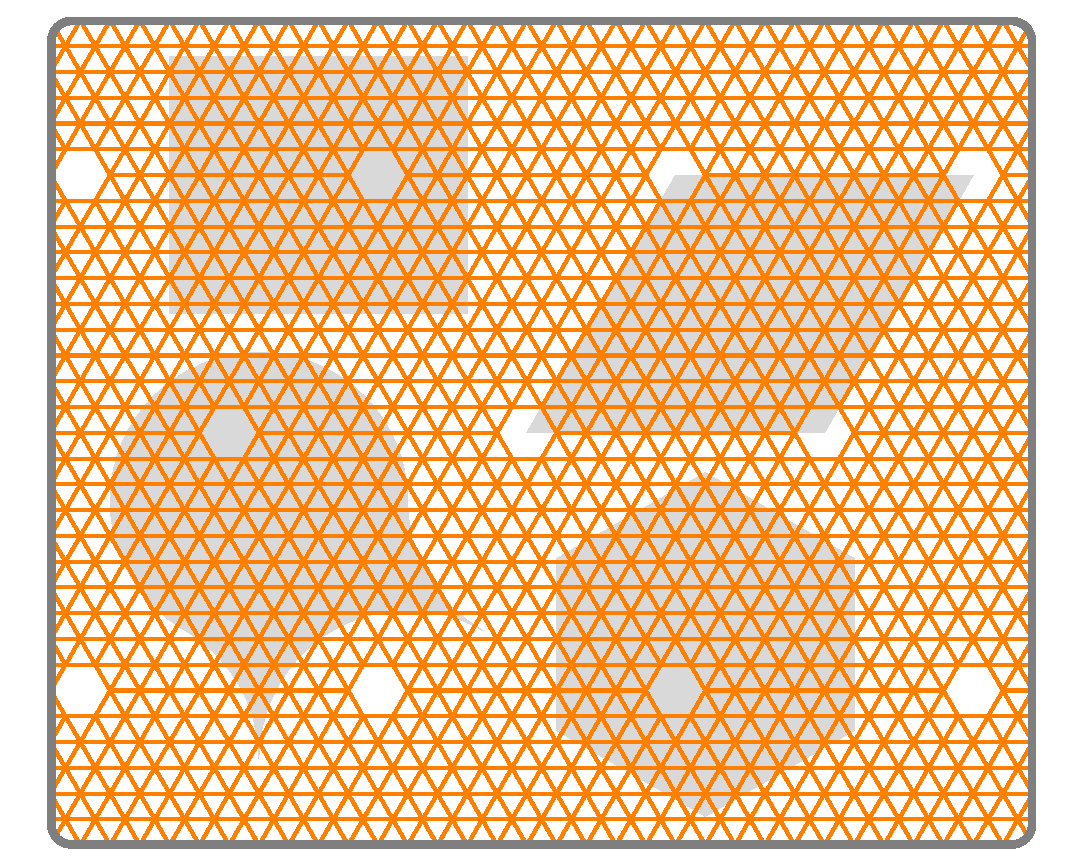
\includegraphics[width=120mm]{flat-torus-5.eps}
  \caption{A torus meshed with triangles}
  \label{\numb section 7.\numb fig 6}
\end{figure}

\begin{Verbatim}[commandchars=\\\{\},formatcom=\small\tt,frame=single,
   label=parag-\ref{\numb section 7.\numb parag 9}.cpp,rulecolor=\color{coment},
   baselinestretch=0.94,framesep=2mm                                            ]
   \verm{Manifold}::Action \azul{g1} ( \textcolor{tag}{tag}::transforms, xy, \textcolor{tag}{tag}::into, (x+1.) && y ),
                    \azul{g2} ( \textcolor{tag}{tag}::transforms, xy, \textcolor{tag}{tag}::into, (x+0.5) && (y+0.866) );
   \verm{Manifold} \azul{torus_manif} = RR2 .quotient ( g1, g2 );
   \verm{Cell} \azul{A} ( \textcolor{tag}{tag}::vertex );  x (A) = 0.;  y (A) = 0.;
   \verm{Mesh} \azul{seg_horiz} ( \textcolor{tag}{tag}::segment, A .reverse(), A,
                    \textcolor{tag}{tag}::divided_in, 10, \textcolor{tag}{tag}::winding, g1 ),
        \azul{seg1}      ( \textcolor{tag}{tag}::segment, A .reverse(), A,
                    \textcolor{tag}{tag}::divided_in, 10, \textcolor{tag}{tag}::winding, g2 ),
        \azul{seg2}      ( \textcolor{tag}{tag}::segment, A .reverse(), A,
                    \textcolor{tag}{tag}::divided_in, 10, \textcolor{tag}{tag}::winding, g2 - g1 );
   \verm{Mesh} \azul{tri1} ( \textcolor{tag}{tag}::triangle, seg_horiz, seg2, seg1 .reverse(), \textcolor{tag}{tag}::winding ),
   \azul{tri2} ( \textcolor{tag}{tag}::triangle, seg_horiz .reverse(), seg2 .reverse(), seg1,
          \textcolor{tag}{tag}::winding                                             );
   \verm{Mesh} \azul{torus} ( \textcolor{tag}{tag}::join, tri1, tri2 );
\end{Verbatim}

Note the additive syntax for composing actions; comments in paragraph
\ref{\numb section 7.\numb parag 3} apply.

In figure \ref{\numb section 7.\numb fig 6} we have drawn four shadows.
The skew paralellogram can be called ``periodicity cell'';
the other three are ``representative domains''.
Due to the shape of one of these shadows, this periodic arrangement is often called
``hexagonal periodicity''.


          %--------%
\section{~~Exercise}\label{\numb section 7.\numb parag 10}
          %--------%

Build the mesh shown in figure \ref{\numb section 7.\numb fig 6}
(the same as in paragraph \ref{\numb section 7.\numb parag 9}) using only one quadrangular patch.
(Hint: have a look at paragraphs \ref{\numb section 2.\numb parag 3} and
\ref{\numb section 2.\numb parag 8}.)


          %----------%
\section{~~A rotation}\label{\numb section 7.\numb parag 11}
          %----------%

Actions are not limited to translations.
Here is an example of a quotient manifold using one rotation.
Note that {\small\tt theta} is not a divisor of $ 2\pi $;
more precisely, no multiple of {\small\tt theta} is a multiple of $ 2\pi $.

It is the user's responsibility to provide an invertible transformation.
In contrast, translations (used in previous paragraphs) are always invertible.

\begin{Verbatim}[commandchars=\\\{\},formatcom=\small\tt,frame=single,
   label=parag-\ref{\numb section 7.\numb parag 11}.cpp,rulecolor=\color{coment},
   baselinestretch=0.94,framesep=2mm                                             ]
   const double \azul{theta} = 1.;  // radians
   const double \azul{cos_theta} = std::cos ( theta ), \azul{sin_theta} = std::sin ( theta );
	
   \cinza{// define an action on RR2 (a rotation)}
   \verm{Manifold}::Action \azul{rot} ( \textcolor{tag}{tag}::transforms, xy, \textcolor{tag}{tag}::into,
         ( cos_theta * x - sin_theta * y ) && ( sin_theta * x + cos_theta * y ) );
   \cinza{// and divide RR2 by the group generated by 'rot'}
   \verm{Manifold} \azul{RR2_q} = RR2 .quotient ( rot );

   \verm{Cell} \azul{A} ( \textcolor{tag}{tag}::vertex );  x(A) = 0.;  y(A) = 1.;
   \verm{Cell} \azul{B} ( \textcolor{tag}{tag}::vertex );  x(B) = 0.;  y(B) = 2.;

   \verm{Mesh} \azul{AA} ( \textcolor{tag}{tag}::segment, A.reverse(), A, \textcolor{tag}{tag}::divided_in, 10, \textcolor{tag}{tag}::winding, -rot );
   \verm{Mesh} \azul{AB} ( \textcolor{tag}{tag}::segment, A.reverse(), B, \textcolor{tag}{tag}::divided_in, 7 );  // no winding
   \verm{Mesh} \azul{BB} ( \textcolor{tag}{tag}::segment, B.reverse(), B, \textcolor{tag}{tag}::divided_in, 10, \textcolor{tag}{tag}::winding, rot );

   \verm{Mesh} \azul{sector} ( \textcolor{tag}{tag}::rectangle, AA, AB, BB, AB .reverse(), \textcolor{tag}{tag}::winding );
\end{Verbatim}

\begin{figure}[ht] \centering
  \psfrag{A}{\small\tt\textcolor{textindraw}{A}}
  \psfrag{B}{\small\tt\textcolor{textindraw}{B}}
  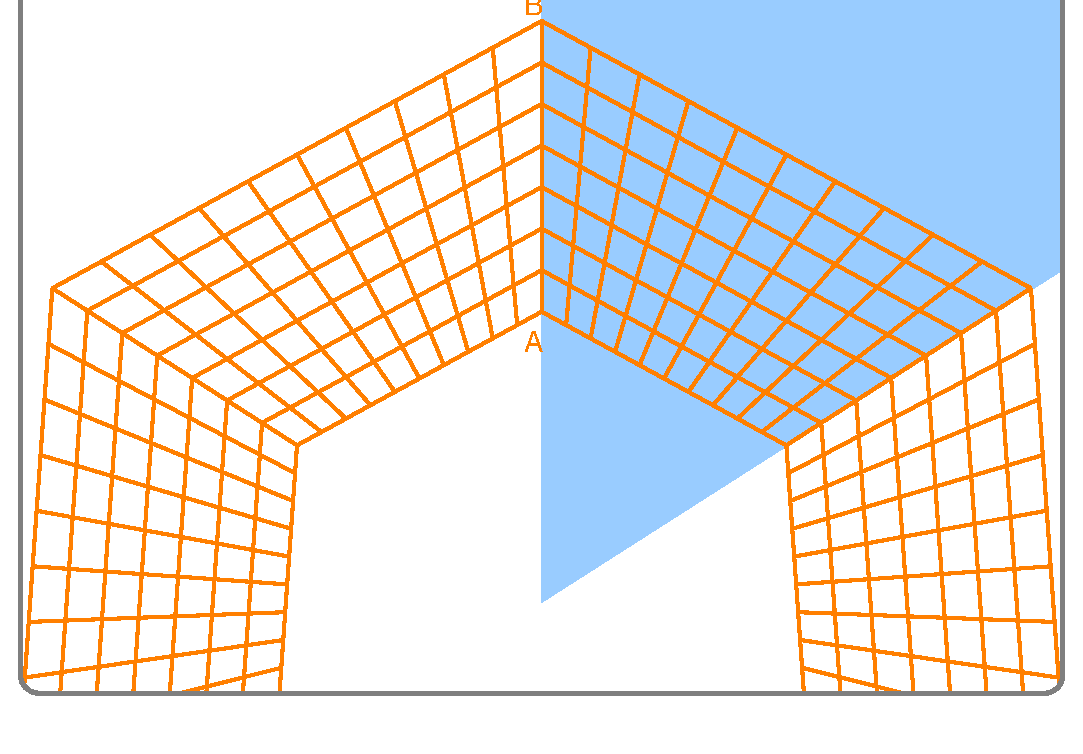
\includegraphics[width=95mm]{sector-1.eps}
  \caption{One rotation}
  \label{\numb section 7.\numb fig 7}
\end{figure}

In figure \ref{\numb section 7.\numb fig 7}
we have drawn a ``representative domain'' but this is not entirely correct since
rotations of this region with multiples of {\small\tt theta} close to $ 2k\pi $
will overlap with the region.

This process is very different from the one described in paragraph
\ref{\numb section 9.\numb parag 2}
where many meshes are built in a {\small\tt for} loop then are joined to form an annulus.


          %----------------%
\section{~~A singular point}\label{\numb section 7.\numb parag 12}
          %----------------%

An interesting question is whether we can extend the mesh up to the origin
(see figure \ref{\numb section 7.\numb fig 7}).
It should be stressed that, when dividing the plane $ \mathbb{R}^2 $ by a rotation,
the origin represents a singularity.
The rotation transforms an ordinay point into a different one,
but the origin is mapped into itself.
This quotient manifold is not locally Euclidian in the neighbourhood of the origin.
The shape of this manifold around the origin is similar to the tip of a cone.
When building a mesh of triangles having the origin as vertex,
we must provide the {\small\tt\textcolor{tag}{tag}::singular}
and {\maniFEM} will take special care with that vertex.

In this paragraph, we build two triangles and then {\small\tt join} them;
figure \ref{\numb section 7.\numb fig 8} shows the unfolded mesh.
The {\small\tt\textcolor{tag}{tag}::singular} is necessary when building
{\small\tt tri\_\,2} but not for {\small\tt tri\_\,1}
because the sides of {\small\tt tri\_\,1} have no winding.
In paragraph \ref{\numb section 7.\numb parag 13}, we use only one triangular mesh.

\begin{figure}[ht] \centering
  \psfrag{O}{\small\tt\textcolor{textindraw}{O}}
  \psfrag{A}{\small\tt\textcolor{textindraw}{A}}
  \psfrag{B}{\small\tt\textcolor{textindraw}{B}}
  \psfrag{S}{\small\tt\textcolor{textindraw}{S}}
  \psfrag{T}{\small\tt\textcolor{textindraw}{T}}
  \psfrag{U}{\small\tt\textcolor{textindraw}{T$^{\mbox{\small\tt *}}$}}
  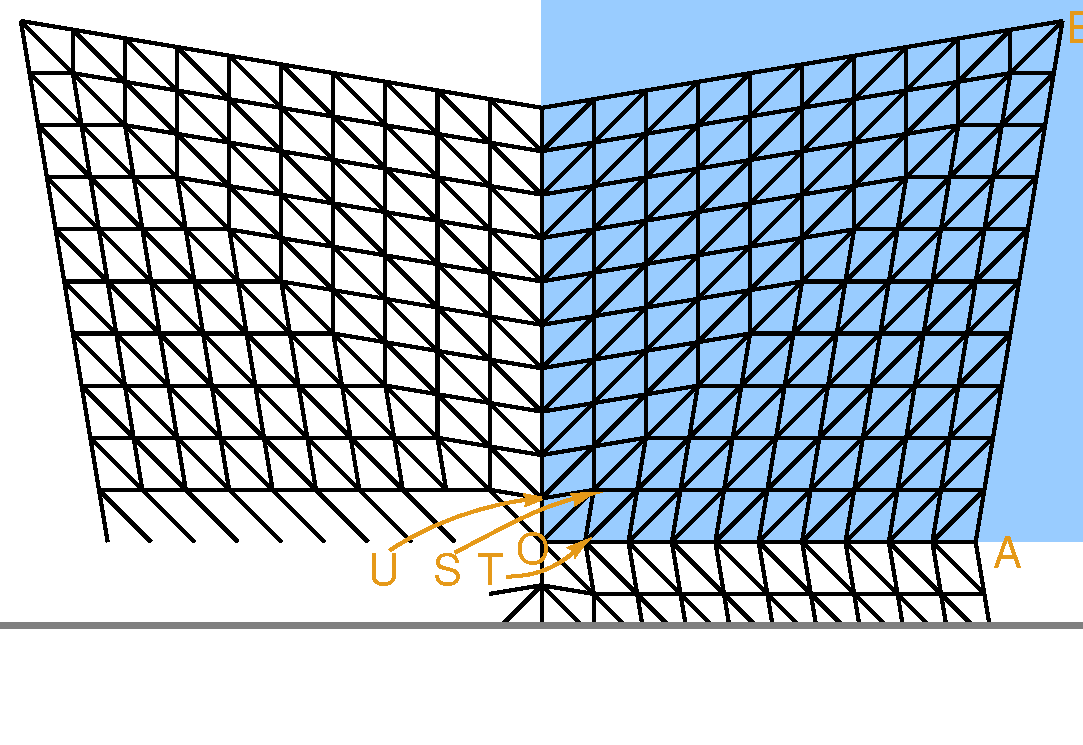
\includegraphics[width=130mm]{butterfly.eps}
  \caption{A vertex similar to the one of a cone}
  \label{\numb section 7.\numb fig 8}
\end{figure}

\begin{Verbatim}[commandchars=\\\{\},formatcom=\small\tt,frame=single,
   label=parag-\ref{\numb section 7.\numb parag 12}.cpp,rulecolor=\color{coment},
   baselinestretch=0.94,framesep=2mm                                             ]
   const double \azul{theta} = pi/2.;  // radians
   const double \azul{cos_theta} = std::cos ( theta ), \azul{sin_theta} = std::sin ( theta );
	
   \cinza{// define an action on RR2 (a rotation)}
   \verm{Manifold}::Action \azul{rot} ( \textcolor{tag}{tag}::transforms, xy, \textcolor{tag}{tag}::into,
         ( cos_theta * x - sin_theta * y ) && ( sin_theta * x + cos_theta * y ) );
   \cinza{// and divide RR2 by the group generated by 'rot'}
   \verm{Manifold} \azul{RR2_q} = RR2 .quotient ( rot );

   \verm{Cell} \azul{O} ( \textcolor{tag}{tag}::vertex );  x (O) = 0. ;  y (O) = 0. ;
   \verm{Cell} \azul{A} ( \textcolor{tag}{tag}::vertex );  x (A) = 1. ;  y (A) = 0. ;
   \verm{Cell} \azul{B} ( \textcolor{tag}{tag}::vertex );  x (B) = 1.2;  y (B) = 1.2;

   \verm{Mesh} \azul{OA} ( \textcolor{tag}{tag}::segment, O .reverse(), A, \textcolor{tag}{tag}::divided_in, 10 );  \cinza{// no winding}
   \verm{Mesh} \azul{OB} ( \textcolor{tag}{tag}::segment, O .reverse(), B, \textcolor{tag}{tag}::divided_in, 10 );  \cinza{// no winding}
   \verm{Mesh} \azul{AB} ( \textcolor{tag}{tag}::segment, A .reverse(), B, \textcolor{tag}{tag}::divided_in, 10 );  \cinza{// no winding}
   \verm{Mesh} \azul{BA} ( \textcolor{tag}{tag}::segment, B .reverse(), A, \textcolor{tag}{tag}::divided_in, 10, \textcolor{tag}{tag}::winding, rot );

   \verm{Mesh} \azul{tri_1} ( \textcolor{tag}{tag}::triangle, OA, AB, OB .reverse() );  \cinza{// no winding}
   \verm{Mesh} \azul{tri_2} ( \textcolor{tag}{tag}::triangle, OB, BA, OA .reverse(),
                \textcolor{tag}{tag}::winding, \textcolor{tag}{tag}::singular, O       );
   \cinza{// on the last triangular cell, the one having O as vertex,}
   \cinza{// the sum of windings is not zero}

   \verm{Mesh} \azul{sector} ( \textcolor{tag}{tag}::join, tri_1, tri_2 );
\end{Verbatim}

Usually, the sum of the winding numbers of the three sides of any triangle is zero.
The triangle last built in this paragraph, {\small\tt OST$^{\mbox{\small\tt *}}$},
does not obey to this rule.


          %-----------------------------%
\section{~~Avoiding degenerate segments}\label{\numb section 7.\numb parag 13}
          %-----------------------------%

In paragraph \ref{\numb section 7.\numb parag 12} we have built two triangular meshes
and then we have {\small\tt join}ed them.

It is possible to build a similar shape with only one triangular mesh.
However, {\maniFEM} cannot build a segment like {\small\tt TT$^{\mbox{\small\tt *}}$},
having the same vertex as base and as tip.
This is why a new vertex is introduced near the origin and the two adjacent triangles
are split (see figure \ref{\numb section 7.\numb fig 9}).

\begin{Verbatim}[commandchars=\\\{\},formatcom=\small\tt,frame=single,
   label=parag-\ref{\numb section 7.\numb parag 13}.cpp,rulecolor=\color{coment},
   baselinestretch=0.94,framesep=2mm                                             ]
   const double \azul{theta} = pi/3.;  // radians
   const double \azul{cos_theta} = std::cos ( theta ), \azul{sin_theta} = std::sin ( theta );
	
   \cinza{// define an action on RR2 (a rotation)}
   \verm{Manifold}::Action \azul{rot} ( \textcolor{tag}{tag}::transforms, xy, \textcolor{tag}{tag}::into,
         ( cos_theta * x - sin_theta * y ) && ( sin_theta * x + cos_theta * y ) );
   \cinza{// and divide RR2 by the group generated by 'rot'}
   \verm{Manifold} \azul{RR2_q} = RR2 .quotient ( rot );

   \verm{Cell} \azul{O} ( \textcolor{tag}{tag}::vertex );  x (O) = 0.;  y (O) = 0.;
   \verm{Cell} \azul{A} ( \textcolor{tag}{tag}::vertex );  x (A) = 1.;  y (A) = 0.;

   \verm{Mesh} \azul{OA} ( \textcolor{tag}{tag}::segment, O .reverse(), A, \textcolor{tag}{tag}::divided_in, 10 );  \cinza{// no winding}
   \verm{Mesh} \azul{AA} ( \textcolor{tag}{tag}::segment, A .reverse(), A, \textcolor{tag}{tag}::divided_in, 10, \textcolor{tag}{tag}::winding, rot );

   \verm{Mesh} \azul{sector} ( \textcolor{tag}{tag}::triangle, OA, AA, OA .reverse(),
                \textcolor{tag}{tag}::winding, \textcolor{tag}{tag}::singular, O         );
\end{Verbatim}

\begin{figure}[ht] \centering
  \psfrag{O}{\small\tt\textcolor{textindraw}{O}}
  \psfrag{A}{\small\tt\textcolor{textindraw}{A}}
  \psfrag{T}{\small\tt\textcolor{textindraw}{T}}
  \psfrag{U}{\small\tt\textcolor{textindraw}{T$^{\mbox{\small\tt *}}$}}
  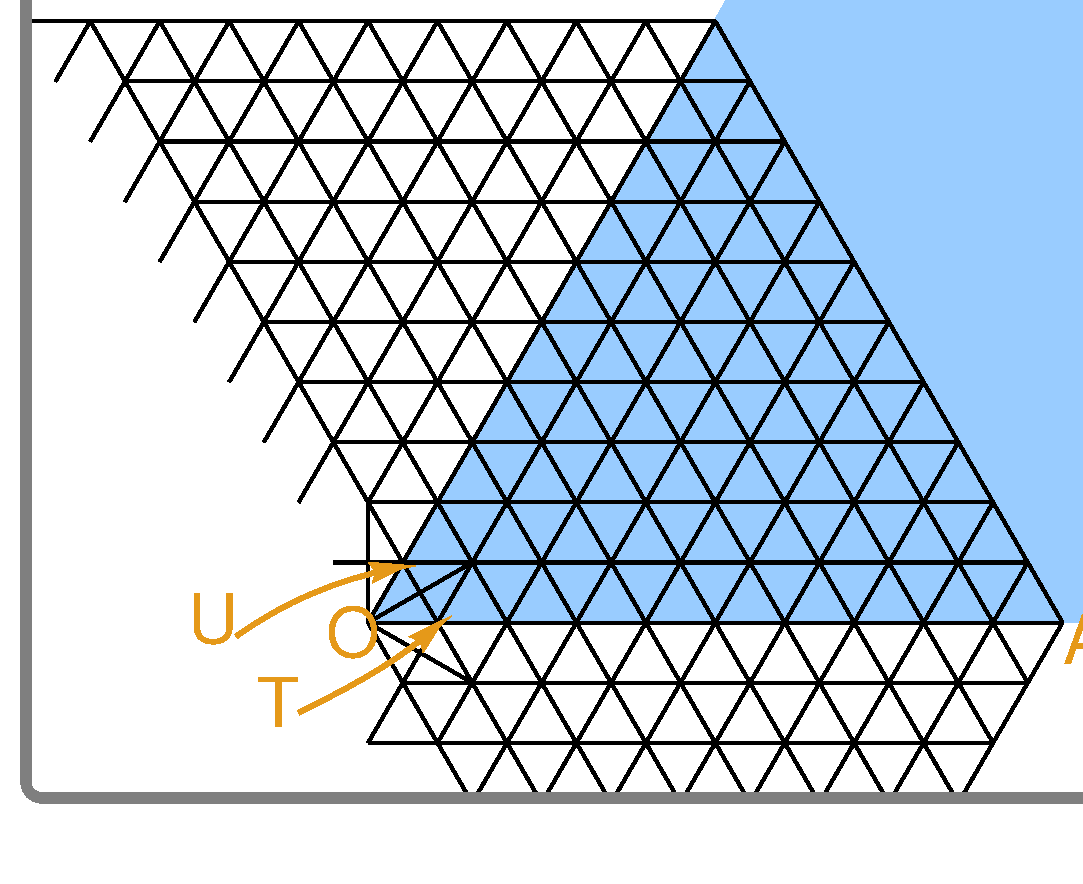
\includegraphics[width=90mm]{sector-cut.eps}
  \caption{A cone-like shape built with one triangular patch}
  \label{\numb section 7.\numb fig 9}
\end{figure}


          %-----------------------%
\section{~~A linear transformation}\label{\numb section 7.\numb parag 14}
          %-----------------------%

Actions can be arbitrary linear transformations.
It is the user's responsibility to provide an invertible transformation.
In contrast, translations are always invertible.

\begin{Verbatim}[commandchars=\\\{\},formatcom=\small\tt,frame=single,
   label=parag-\ref{\numb section 7.\numb parag 14}.cpp,rulecolor=\color{coment},
   baselinestretch=0.94,framesep=2mm                                             ]
   // define an action on RR2 (a linear map)
   \verm{Manifold}::Action \azul{g} ( \textcolor{tag}{tag}::transforms, xy, \textcolor{tag}{tag}::into,
      ( 0.8 * cos_theta * x - 0.8 * sin_theta * y ) &&
      ( 0.8 * sin_theta * x + 0.8 * cos_theta * y )    );

   // and divide RR2 by the group generated by g
   \verm{Manifold} \azul{RR2_q} = RR2 .quotient ( g );
\end{Verbatim}

\begin{figure}[ht] \centering
  \psfrag{A}{\small\tt\textcolor{textindraw}{A}}
  \psfrag{B}{\small\tt\textcolor{textindraw}{B}}
  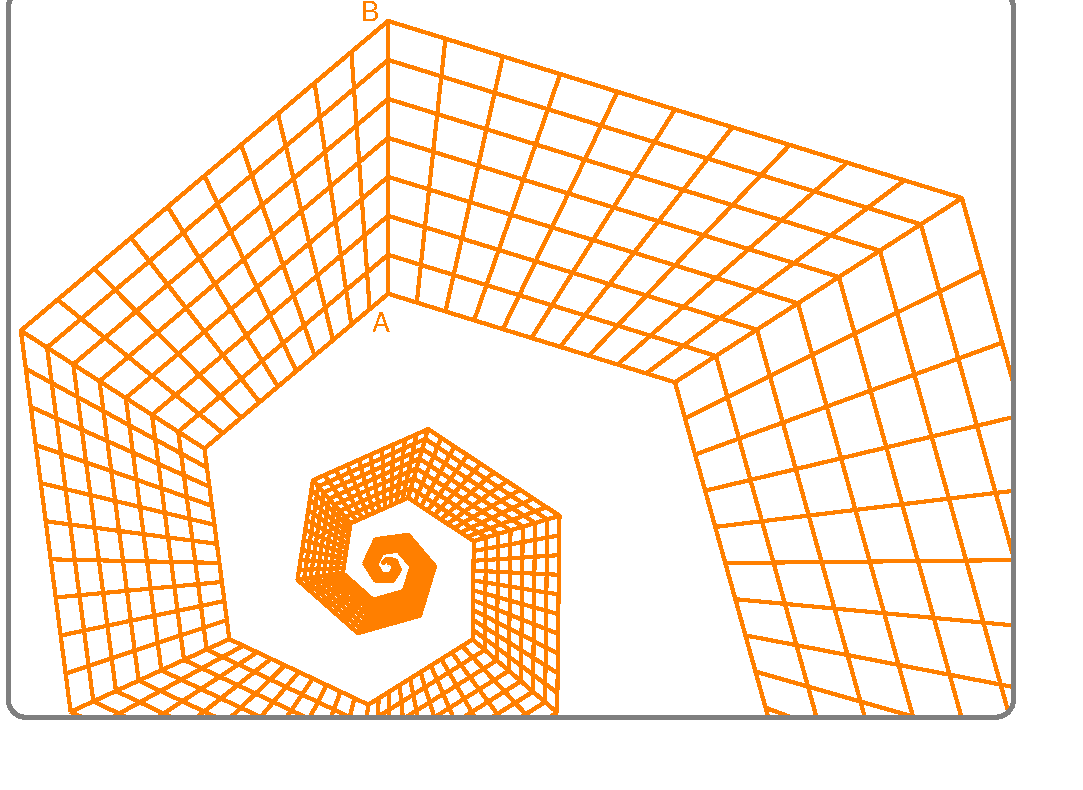
\includegraphics[width=96mm]{sector-2.eps}
  \caption{One linear transformation}
  \label{\numb section 7.\numb fig 10}
\end{figure}

Note that in this example the metric is not well-defined
so the manifold we are dealing with is not a Riemannian manifold.


          %--------------------------%
\section{~~Two linear transformations}\label{\numb section 7.\numb parag 15}
          %--------------------------%

Here is an example with two linear transformations.
It is the user's responsibility to provide invertible transformations and
to make sure that they commute.
In contrast, translations are always invertible and they commute.

\begin{Verbatim}[commandchars=\\\{\},formatcom=\small\tt,frame=single,
   label=parag-\ref{\numb section 7.\numb parag 15}.cpp,rulecolor=\color{coment},
   baselinestretch=0.94,framesep=2mm                                             ]
   // define two actions on RR2
   // a rotation
   \verm{Manifold}::Action \azul{rot} ( \textcolor{tag}{tag}::transforms, xy, \textcolor{tag}{tag}::into,
      ( cos_theta * x - sin_theta * y ) && ( sin_theta * x + cos_theta * y ) );
   // and a zoom
   \verm{Manifold}::Action \azul{zoom} ( \textcolor{tag}{tag}::transforms, xy, \textcolor{tag}{tag}::into, ( 2.*x ) && ( 2.*y ) );

   // divide RR2 by the group generated by \{ rot, zoom \}
   \verm{Manifold} \azul{torus_manif} = RR2 .quotient ( rot, zoom );

   // one vertex is enough to start the process
   \verm{Cell} \azul{A} ( \textcolor{tag}{tag}::vertex );  x (A) = 0.;  y (A) = 1.;
   \verm{Mesh} \azul{AA} ( \textcolor{tag}{tag}::segment, A.reverse(), A, \textcolor{tag}{tag}::divided_in, 10, \textcolor{tag}{tag}::winding, -rot );
   \verm{Mesh} \azul{AA_vert} ( \textcolor{tag}{tag}::segment, A .reverse(), A,
                  \textcolor{tag}{tag}::divided_in, 7, \textcolor{tag}{tag}::winding, zoom );

   \verm{Mesh} \azul{sector} ( \textcolor{tag}{tag}::rectangle, AA, AA_vert, AA .reverse(), AA_vert .reverse(),
                 \textcolor{tag}{tag}::winding                                                   );
\end{Verbatim}
  
\begin{figure}[ht] \centering
  \psfrag{A}{\small\tt\textcolor{textindraw}{A}}
  \psfrag{B}{\small\tt\textcolor{textindraw}{B}}
  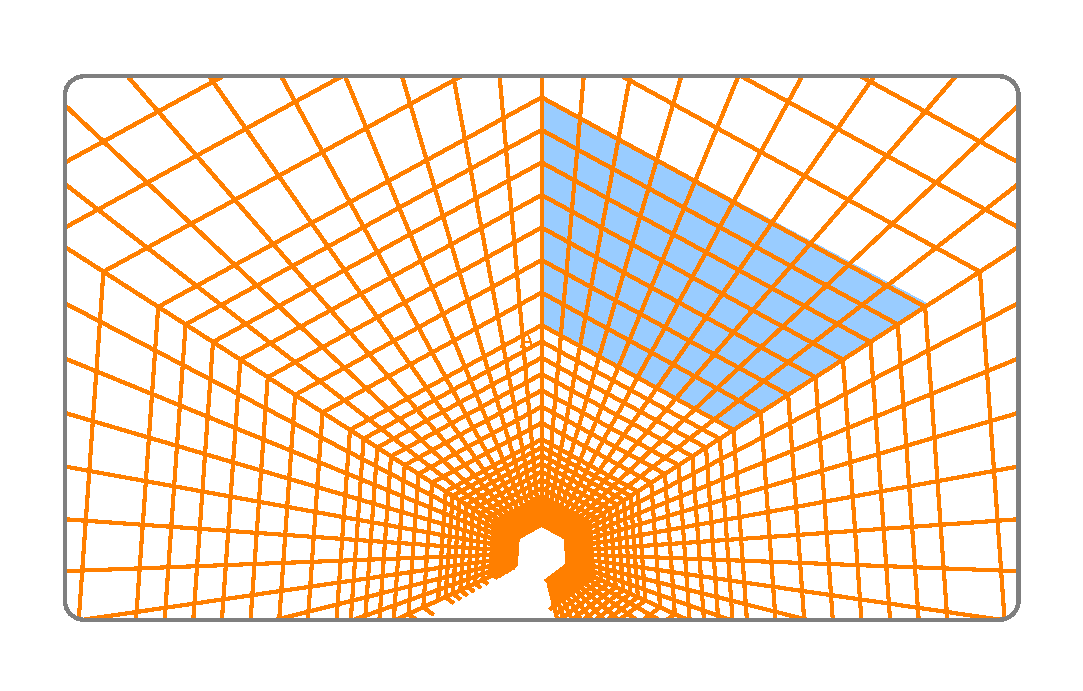
\includegraphics[width=100mm]{sector-3.eps}
  \caption{Two linear transformations : a rotation and a zoom}
  \label{\numb section 7.\numb fig 11}
\end{figure}

Again, the metric is not well-defined (due to the zoom)
so the manifold we are dealing with is not a Riemannian manifold.


          %---------------------------------%
\section{~~Wrapping a mesh around a cylinder}\label{\numb section 7.\numb parag 16}
          %---------------------------------%

We can start with a usual mesh in the Euclidian plane and wrap it around a cylinder.
Or we may call this operation ``wind'' or ``fold''.
The outer boundary of the mesh must have two parallel segments of equal length and with
the same number of segments (to be identified).
The mesh may have many other details (like the circular hole shown in figure
\ref{\numb section 7.\numb fig 11}) which do not interfere in the process.

\begin{Verbatim}[commandchars=\\\{\},formatcom=\small\tt,frame=single,
   label=parag-\ref{\numb section 7.\numb parag 16}.cpp,rulecolor=\color{coment},
   baselinestretch=0.94,framesep=2mm                                             ]
   \verm{Manifold} \azul{RR2} ( \textcolor{tag}{tag}::Euclid, \textcolor{tag}{tag}::of_dim, 2 );
   \verm{Function} \azul{xy} = RR2 .build_coordinate_system ( \textcolor{tag}{tag}::Lagrange, \textcolor{tag}{tag}::of_degree, 1 );
   \verm{Function} \azul{x} = xy [0], \azul{y} = xy [1];

   size_t \azul{n} = 20;
   double \azul{d} = 2.6 / double(n);

   \verm{Cell} \azul{A} ( \textcolor{tag}{tag}::vertex );  x (A) = -1.3;  y (A) = -1.3;
   \verm{Cell} \azul{B} ( \textcolor{tag}{tag}::vertex );  x (B) =  1.3;  y (B) = -1.3;
   \verm{Cell} \azul{C} ( \textcolor{tag}{tag}::vertex );  x (C) =  1.3;  y (C) =  1.3;
   \verm{Cell} \azul{D} ( \textcolor{tag}{tag}::vertex );  x (D) = -1.3;  y (D) =  1.3;

   \verm{Mesh} \azul{AB} ( \textcolor{tag}{tag}::segment, A .reverse(), B, \textcolor{tag}{tag}::divided_in, n );
   \verm{Mesh} \azul{BC} ( \textcolor{tag}{tag}::segment, B .reverse(), C, \textcolor{tag}{tag}::divided_in, n );
   \verm{Mesh} \azul{CD} ( \textcolor{tag}{tag}::segment, C .reverse(), D, \textcolor{tag}{tag}::divided_in, n );
   \verm{Mesh} \azul{DA} ( \textcolor{tag}{tag}::segment, D .reverse(), A, \textcolor{tag}{tag}::divided_in, n );

   \verm{Manifold} \azul{circle} = RR2 .implicit ( x*x + y*y == 1. );
   \verm{Mesh} \azul{inner}
      ( \textcolor{tag}{tag}::progressive, \textcolor{tag}{tag}::entire_manifold, circle, \textcolor{tag}{tag}::desired_length, d );

   \verm{Mesh} \azul{bdry} ( \textcolor{tag}{tag}::join, AB, BC, CD, DA, inner .reverse() );
   RR2.set_as_working_manifold();
   \verm{Mesh} \azul{square} ( \textcolor{tag}{tag}::progressive, \textcolor{tag}{tag}::boundary, bdry, \textcolor{tag}{tag}::desired_length, d );

   \verm{Mesh} \azul{cyl} = square .fold
      ( \textcolor{tag}{tag}::identify, BC, \textcolor{tag}{tag}::with, DA .reverse(), \textcolor{tag}{tag}::use_existing_vertices );
\end{Verbatim}

The method {\small\tt\verm{Mesh}::fold} (which can also be used under the names
{\small\tt\verm{Mesh}::wrap} or {\small\tt\verm{Mesh}::wind}) uses information
from the geometry of the mesh to identify an action defining a periodicity group,
builds a quotient manifold using this action then builds a new mesh on this quotient manifold
by identifying the specified pair of segment meshes.

\begin{figure}[ht] \centering
  \psfrag{A}{\small\tt\textcolor{textindraw}{A}}
  \psfrag{B}{\small\tt\textcolor{textindraw}{B}}
  \psfrag{C}{\small\tt\textcolor{textindraw}{C}}
  \psfrag{D}{\small\tt\textcolor{textindraw}{D}}
  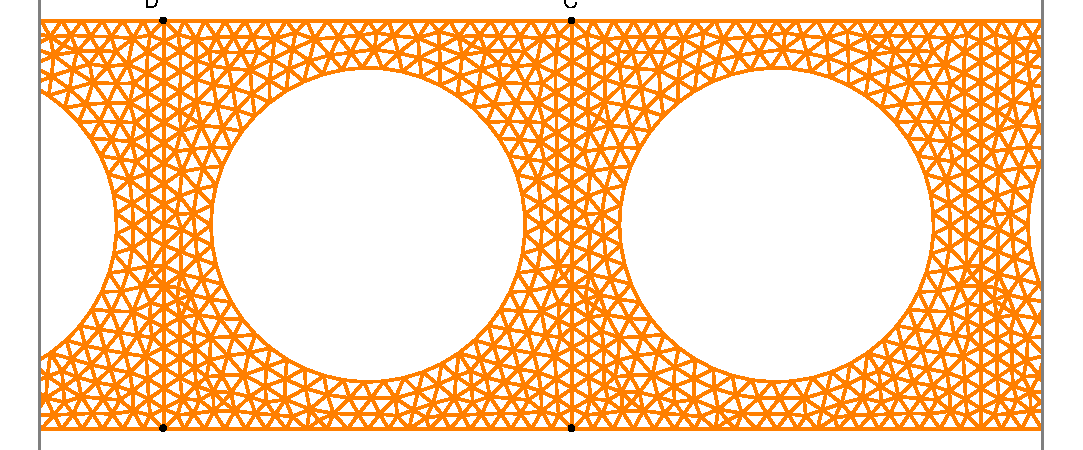
\includegraphics[width=120mm]{cylinder-1.eps}
  \caption{Identifying a pair of opposite faces}
  \label{\numb section 7.\numb fig 12}
\end{figure}

The mesh {\small\tt\azul{cyl}} is entirely new and distinct from {\small\tt square},
with the exception of vertices, which can be shared between the two meshes if the
user so desires.
The last argument of method {\small\tt\verm{Mesh}::fold} controls this detail.
A {\small\tt\textcolor{tag}{tag}::build\_\,new\_\,vertices} says that new vertices must be built
and geometric coordinates copied from the old vertices to the new ones.
A {\small\tt\textcolor{tag}{tag}::use\_\,existing\_\,vertices} says that old vertices
should be used for the new mesh; this can be useful if the vertices carry some information
(e.g.\ values of a solution of a PDE) and also saves space in the computer's memory.
Note that vertices belonging to {\small\tt DA} will not show up in the
new mesh; corresponding vertices from {\small\tt BC} will be used instead.

We must identify {\small\tt BC} with the reverse of {\small\tt DA} (which we may call
{\small\tt AD} if we wish); trying to identify {\small\tt BC} with {\small\tt DA} should
result in a twisted cylinder (a M\"obius strip) but {\maniFEM} will reject such a construction.
This event is discussed in paragraph \ref{\numb section 13.\numb parag 5}.


          %------------------------------%
\section{~~Wrapping a mesh around a torus}\label{\numb section 7.\numb parag 17}
          %------------------------------%

A process similar to the one described in paragraph \ref{\numb section 7.\numb parag 16}
can be used to ``wrap'' a mesh (having a parallelogram as outer boundary) around
a torus.
It suffices to identify two pairs of opposite faces.

\begin{Verbatim}[commandchars=\\\{\},formatcom=\small\tt,frame=single,
   label=parag-\ref{\numb section 7.\numb parag 17}.cpp,rulecolor=\color{coment},
   baselinestretch=0.94,framesep=2mm                                             ]
   \verm{Mesh} \azul{torus} = square .fold ( \textcolor{tag}{tag}::identify, AB, \textcolor{tag}{tag}::with, CD .reverse(),
                               \textcolor{tag}{tag}::identify, BC, \textcolor{tag}{tag}::with, DA .reverse(),
                               \textcolor{tag}{tag}::use_existing_vertices                  );
\end{Verbatim}


          %--------------------------------%
\section{~~Identifying three pairs of sides}\label{\numb section 7.\numb parag 18}
          %--------------------------------%

If we want to obtain the hexagonal periodicity referred in paragraph
\ref{\numb section 7.\numb parag 9}, we can literally take a hexagon and
identify three pairs of opposite faces.
Actually, we can even take a rectangle%
\footnote{This rectangle is somewhat similar to the square in paragraph
\ref{\numb section 7.\numb parag 8}.
It is different in that it has a round hole and different aspect ratio --
it has the proportions of the rectangular shadow in figure \ref{\numb section 7.\numb fig 6}.}
and treat it as if it were a hexagon :

\begin{Verbatim}[commandchars=\\\{\},formatcom=\small\tt,frame=single,
   label=parag-\ref{\numb section 7.\numb parag 18}.cpp,rulecolor=\color{coment},
   baselinestretch=0.94,framesep=2mm                                             ]
   const double \azul{d} = 0.13;
   const size_t \azul{n} = 1.5 / d, \azul{m} = 2.6 / d;

   \verm{Cell} \azul{A} ( \textcolor{tag}{tag}::vertex );  x (A) = -1.5;  y (A) = -1.3;
   \verm{Cell} \azul{B} ( \textcolor{tag}{tag}::vertex );  x (B) =  0. ;  y (B) = -1.3;
   \verm{Cell} \azul{C} ( \textcolor{tag}{tag}::vertex );  x (C) =  1.5;  y (C) = -1.3;
   \verm{Cell} \azul{D} ( \textcolor{tag}{tag}::vertex );  x (D) =  1.5;  y (D) =  1.3;
   \verm{Cell} \azul{E} ( \textcolor{tag}{tag}::vertex );  x (E) =  0. ;  y (E) =  1.3;
   \verm{Cell} \azul{F} ( \textcolor{tag}{tag}::vertex );  x (F) = -1.5;  y (F) =  1.3;

   \verm{Mesh} \azul{AB} ( \textcolor{tag}{tag}::segment, A .reverse(), B, \textcolor{tag}{tag}::divided_in, n );
   \verm{Mesh} \azul{BC} ( \textcolor{tag}{tag}::segment, B .reverse(), C, \textcolor{tag}{tag}::divided_in, n );
   \verm{Mesh} \azul{CD} ( \textcolor{tag}{tag}::segment, C .reverse(), D, \textcolor{tag}{tag}::divided_in, m );
   \verm{Mesh} \azul{DE} ( \textcolor{tag}{tag}::segment, D .reverse(), E, \textcolor{tag}{tag}::divided_in, n );
   \verm{Mesh} \azul{EF} ( \textcolor{tag}{tag}::segment, E .reverse(), F, \textcolor{tag}{tag}::divided_in, n );
   \verm{Mesh} \azul{FA} ( \textcolor{tag}{tag}::segment, F .reverse(), A, \textcolor{tag}{tag}::divided_in, m );

   \verm{Manifold} \azul{circle} = RR2 .implicit ( x*x + y*y == 1. );
   \verm{Mesh} \azul{inner} ( \textcolor{tag}{tag}::progressive, \textcolor{tag}{tag}::entire_manifold, circle,
                \textcolor{tag}{tag}::desired_length, d                         );

   \verm{Mesh} \azul{bdry} ( \textcolor{tag}{tag}::join, { AB, BC, CD, DE, EF, FA, inner .reverse() } );
   RR2.set_as_working_manifold();
   \verm{Mesh} \azul{rectangle} ( \textcolor{tag}{tag}::progressive, \textcolor{tag}{tag}::boundary, bdry, \textcolor{tag}{tag}::desired_length, d );
\end{Verbatim}

\begin{figure}[ht] \centering
  \psfrag{A}{\small\tt\textcolor{textindraw}{A}}
  \psfrag{B}{\small\tt\textcolor{textindraw}{B}}
  \psfrag{C}{\small\tt\textcolor{textindraw}{C}}
  \psfrag{D}{\small\tt\textcolor{textindraw}{D}}
  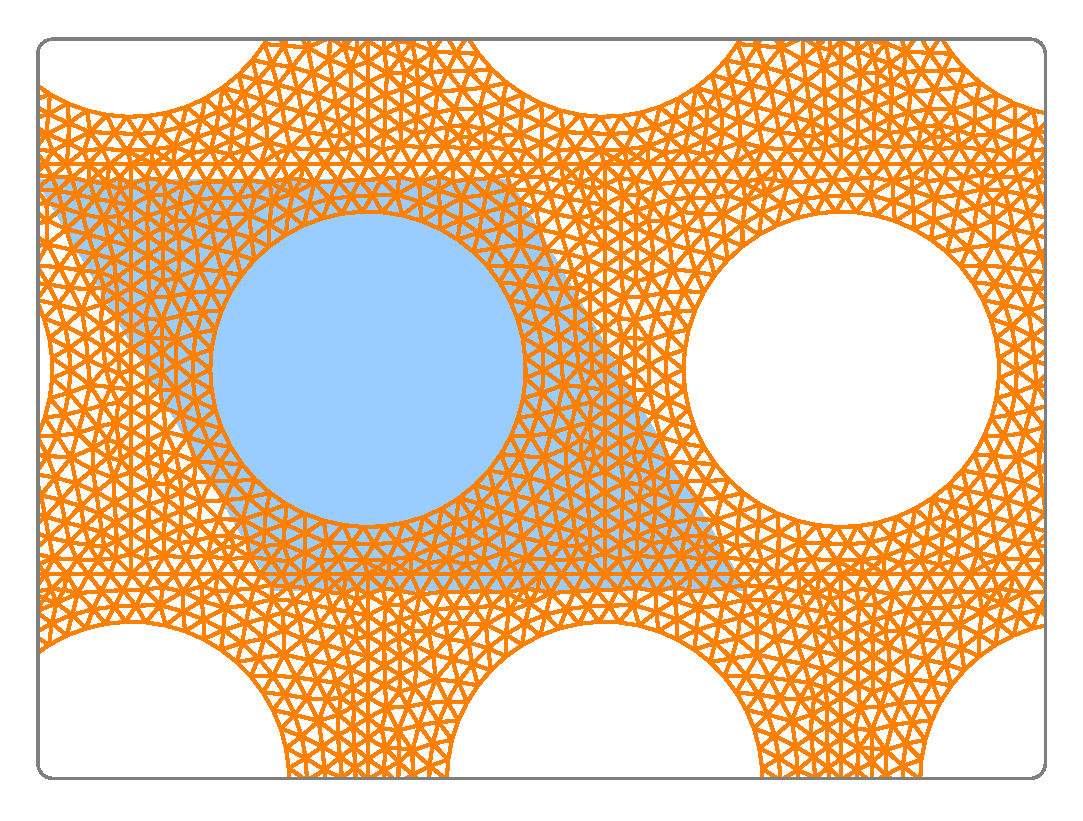
\includegraphics[width=135mm]{hexa-round-hole.eps}
  \caption{Hexagonal arrangement of a circular hole}
  \label{\numb section 7.\numb fig 13}
\end{figure}

\begin{Verbatim}[commandchars=\\\{\},formatcom=\small\tt,frame=single,
   label=parag-\ref{\numb section 7.\numb parag 18}.cpp,rulecolor=\color{coment},
   baselinestretch=0.94,framesep=2mm                                             ]
   \verm{Mesh} \azul{torus} = rectangle .fold ( \textcolor{tag}{tag}::identify, CD, \textcolor{tag}{tag}::with, FA .reverse(),
                                  \textcolor{tag}{tag}::identify, BC, \textcolor{tag}{tag}::with, EF .reverse(),
                                  \textcolor{tag}{tag}::identify, AB, \textcolor{tag}{tag}::with, DE .reverse(),
                                  \textcolor{tag}{tag}::use_existing_vertices                  );
\end{Verbatim}

Figure \ref{\numb section 7.\numb fig 13} shows the resulting mesh, together with the
periodicity cell.
We recall that the same periodicity group (i.e., periodic arrangement) may be generated
by different sets of generators and, consequently, may be viewed as originating
from different periodicity cells.


                 %-----------------------------------------%
\section{~~\cinza{Progressive meshing on quotient manifolds}}
                 %-----------------------------------------%
\label{\numb section 7.\numb parag 19}

\vskip 2mm plus 2mm
{\normalfont\bfseries The code described in this paragraph does not work yet.
It should be regarded as a mere declaration of intentions.}
\medskip
\vskip 3mm plus 2mm

The algorithm for progressive meshing (described in section \ref{\numb section 3})
should work on quotient manifolds with only minimal changes.
Here is how we see it working in the future.

We begin by defining two closed curves (the boundaries of the two future holes),
represented in Figure \ref{\numb section 7.\numb fig 14}.
We use one-dimensional submanifolds of the Euclidian plane $ \mathbb{R}^2 $.

\begin{Verbatim}[commandchars=\\\{\},formatcom=\small\tt,frame=single,
   rulecolor=\color{coment},baselinestretch=0.94,framesep=2mm         ]
   \verm{Manifold} \azul{RR2} ( \textcolor{tag}{tag}::Euclid, \textcolor{tag}{tag}::of_dim, 2 );
   \verm{Function} \azul{xy} = RR2 .build_coordinate_system ( \textcolor{tag}{tag}::Lagrange, \textcolor{tag}{tag}::of_degree, 1 );
   \verm{Function} \azul{x} = xy [0], \azul{y} = xy [1];
   
   const double \azul{e} = 1.5;
   \verm{Manifold} \azul{curve1} = RR2 .implicit 
      ( \verm{smooth_min} ( 300.*\verm{power}((x+y)*(x+y),e) + \verm{power}((x-y-1.)*(x-y-1.),e),
                     300.*\verm{power}((x-y)*(x-y),e) + \verm{power}((x+y+1.)*(x+y+1.),e),
                     \textcolor{tag}{tag}::threshold, 1.5                     )  == 1. );
   \verm{Mesh} \azul{loop1} ( \textcolor{tag}{tag}::progressive, \textcolor{tag}{tag}::desired_length, 0.05 );
      
   double \azul{a} = 0.15, \azul{b} = 0.82;
   \verm{Manifold} \azul{curve2} = RR2 .implicit 
      ( \verm{smooth_min} ( 300.*\verm{power}((x-a+y+b)*(x-a+y+b),e) +
                          \verm{power}((x-a-y-b-1.)*(x-a-y-b-1.),e),
                     300.*\verm{power}((x-2.-a-y-b)*(x-2.-a-y-b),e) +
                          \verm{power}((x-2.-a+y+b+1.)*(x-2.-a+y+b+1.),e),
                     \textcolor{tag}{tag}::threshold, 1.5                           )  == 1. );
   \verm{Mesh} \azul{loop2} ( \textcolor{tag}{tag}::progressive, \textcolor{tag}{tag}::desired_length, 0.05 );

   \verm{Mesh} \azul{loops} ( \textcolor{tag}{tag}::join, loop1 .reverse(), loop2 .reverse() );                     
\end{Verbatim}

\begin{figure}[ht] \centering
  \psfrag{A}{\small\tt\textcolor{textindraw}{A}}
  \psfrag{B}{\small\tt\textcolor{textindraw}{B}}
  \psfrag{C}{\small\tt\textcolor{textindraw}{C}}
  \psfrag{D}{\small\tt\textcolor{textindraw}{D}}
  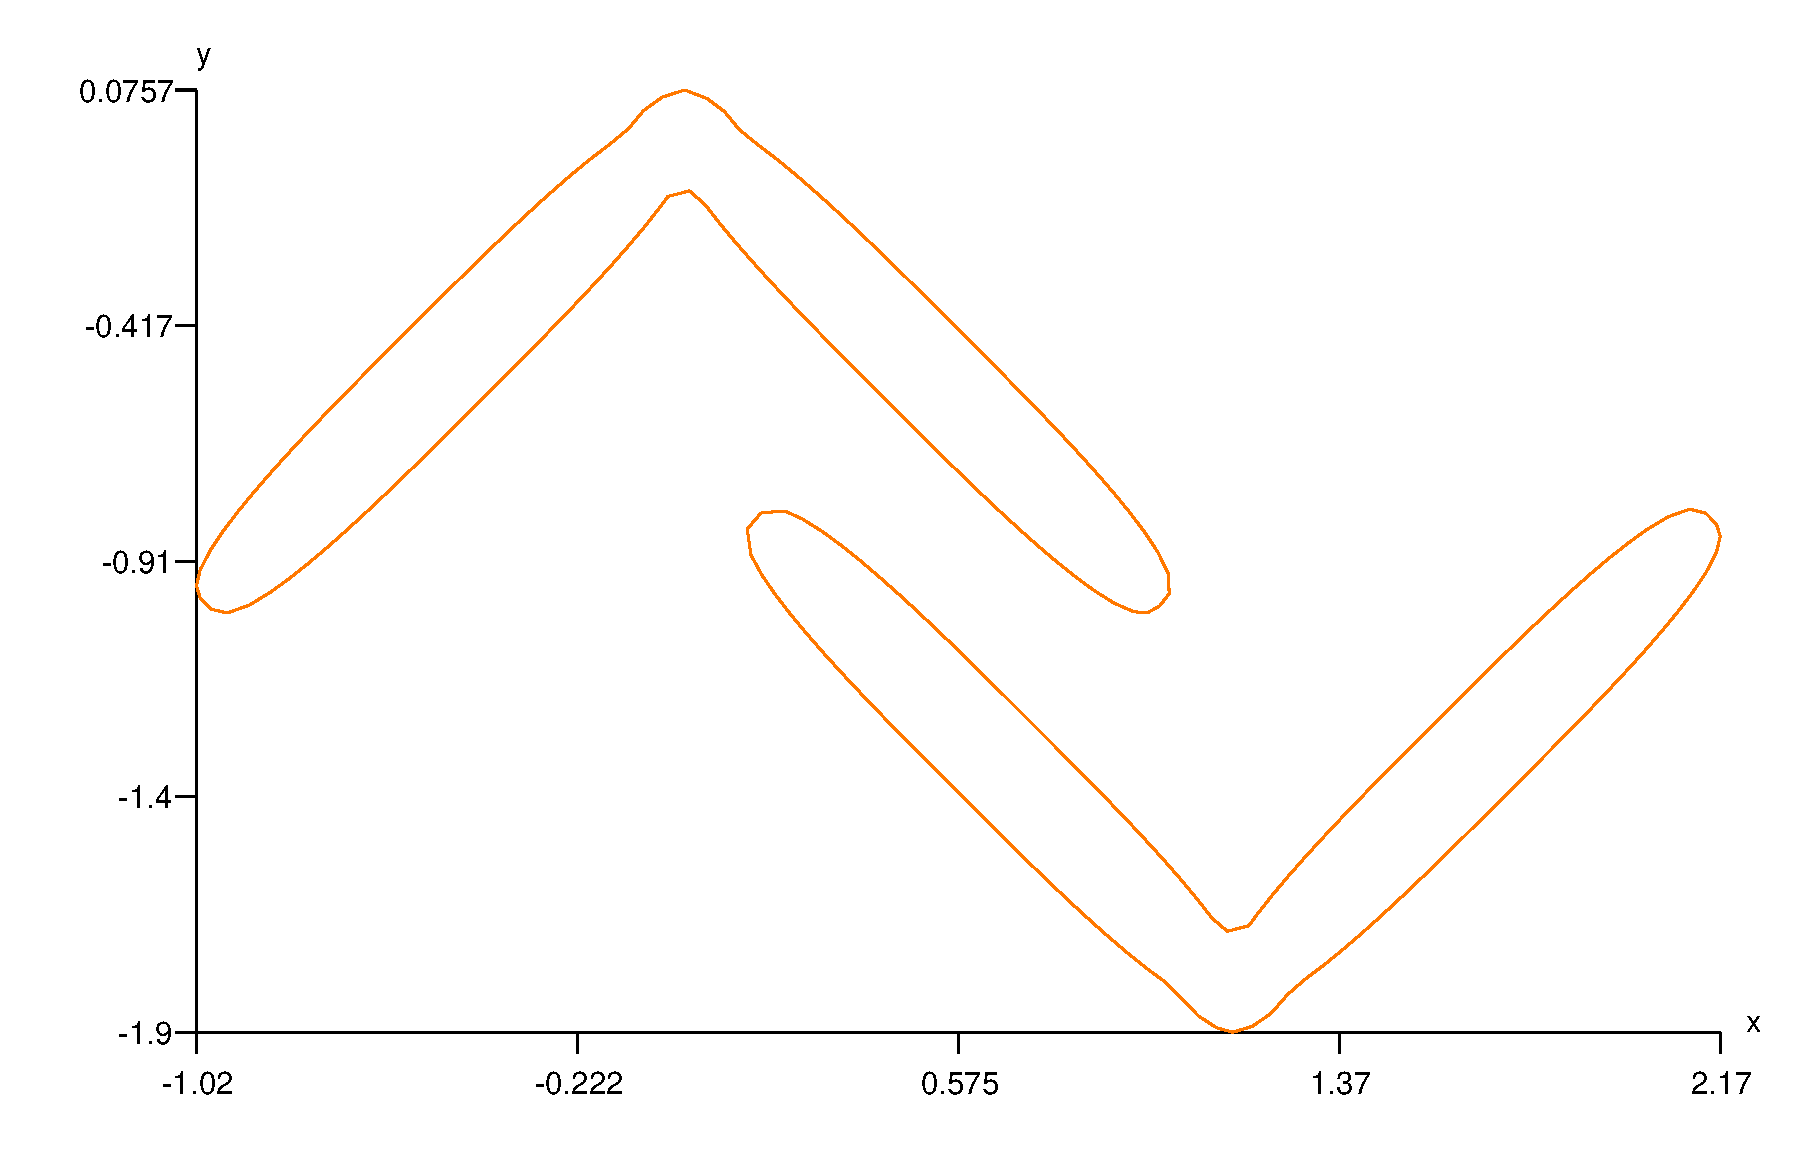
\includegraphics[width=90mm]{boomerang-1.eps}
  \caption{Two V-shaped loops}
  \label{\numb section 7.\numb fig 14}
\end{figure}

The {\small\tt loops} are reversed because they are going to be boundaries of holes
in the mesh (the mesh will be on the exterior of each curve).

Define a torus manifold by means of two appropriate translations.

\begin{Verbatim}[commandchars=\\\{\},formatcom=\small\tt,frame=single,
   rulecolor=\color{coment},baselinestretch=0.94,framesep=2mm         ]
   \verm{Manifold}::Action \azul{g1} ( \textcolor{tag}{tag}::transforms, xy, \textcolor{tag}{tag}::into, (x+2.3) && y ),
                    \azul{g2} ( \textcolor{tag}{tag}::transforms, xy, \textcolor{tag}{tag}::into, x && (y+1.4) );
   \verm{Manifold} \azul{torus_manif} = RR2 .quotient ( g1, g2 );
\end{Verbatim}

\vskip -2mm
Then, fold the two curves around this torus; the result is shown (after unfolding) in figure
\ref{\numb section 7.\numb fig 15}.
Calling the {\small\tt\verm{Mesh}::fold} method with only one argument is quite different
from what we have seen in paragraphs \ref{\numb section 7.\numb parag 16} and
\ref{\numb section 7.\numb parag 17}.
There, the geometry of the manifold (the actions defining the group) were computed from
the geometry of the given mesh.
Here, it is the other way around : a quotient manifold has already been declared and
the folding operation will use the geometry of this torus.

\begin{Verbatim}[commandchars=\\\{\},formatcom=\small\tt,frame=single,
   rulecolor=\color{coment},baselinestretch=0.94,framesep=2mm         ]
   \verm{Mesh} \azul{folded_loops} = loops .fold ( \textcolor{tag}{tag}::use_existing_vertices );
   folded_loops .draw_ps (\verde{"VV.eps"}, \textcolor{tag}{tag}::unfold,
                           \textcolor{tag}{tag}::over_region, -1.5 < x < 2.5, -2 < y < 0.5 );
\end{Verbatim}

\begin{figure}[ht] \centering
  \psfrag{A}{\small\tt\textcolor{textindraw}{A}}
  \psfrag{B}{\small\tt\textcolor{textindraw}{B}}
  \psfrag{C}{\small\tt\textcolor{textindraw}{C}}
  \psfrag{D}{\small\tt\textcolor{textindraw}{D}}
  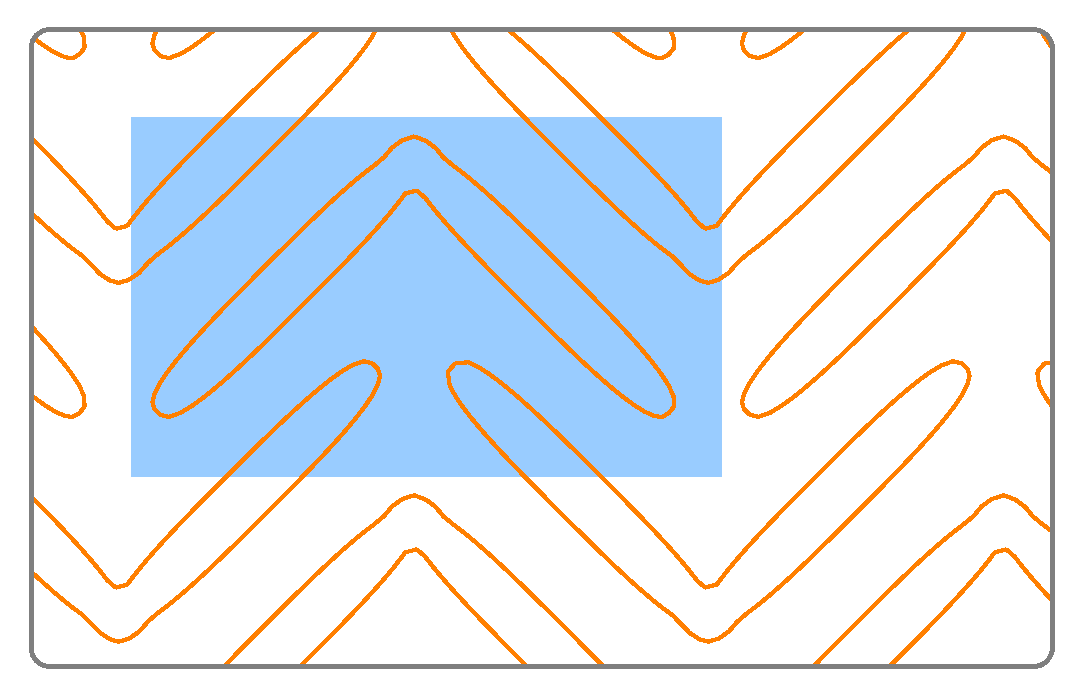
\includegraphics[width=90mm]{boomerang-2.eps}
  \caption{Two V-shaped loops, folded then unfolded}
  \label{\numb section 7.\numb fig 15}
\end{figure}

When we declare the {\small\tt\azul{torus\_\,manif}}, we must use translations chosen with care,
avoiding intersections of these curves with themselves or with each other during the subsequent
\mbox{{\small\tt fold\hskip 0.2 pt}ing}.
\ManiFEM{} does not check for such intersections, it is the user's resposibility to avoid them.

Now call the progressive meshing algorithm.
The algorithm starts from the given boundary and creates new triangles until
it meets the mesh on the other side of the torus.

\begin{Verbatim}[commandchars=\\\{\},formatcom=\small\tt,frame=single,
   label=code not working,rulecolor=\color{coment},
   baselinestretch=0.94,framesep=2mm                                   ]
   \verm{Mesh} \azul{perforated} ( \textcolor{tag}{tag}::progressive, \textcolor{tag}{tag}::boundary, loops,
                     \textcolor{tag}{tag}::desired_length, 0.05              );
   perforated .draw_ps (\verde{"perforated.eps"}, \textcolor{tag}{tag}::unfold,
                         \textcolor{tag}{tag}::over_region, -1.5 < x < 2.5, -2 < y < 0.5 );
\end{Verbatim}

\begin{figure}[ht] \centering
  \psfrag{A}{\small\tt\textcolor{textindraw}{A}}
  \psfrag{B}{\small\tt\textcolor{textindraw}{B}}
  \psfrag{C}{\small\tt\textcolor{textindraw}{C}}
  \psfrag{D}{\small\tt\textcolor{textindraw}{D}}
  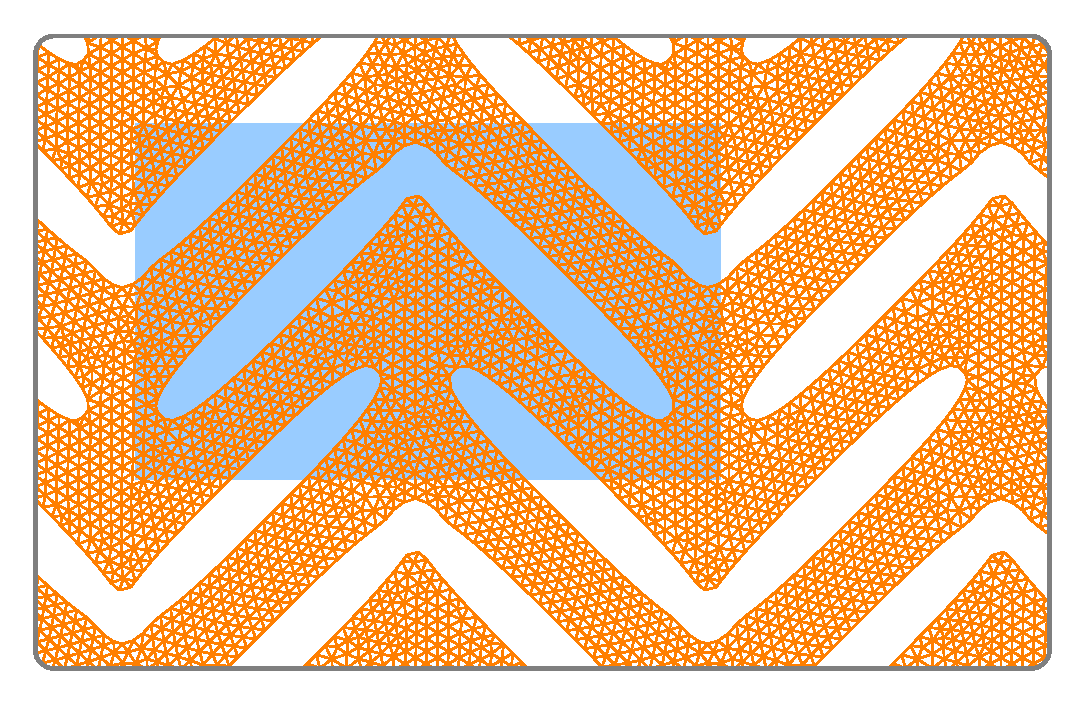
\includegraphics[width=140mm]{boomerang-3.eps}
  \caption{Periodically perforated plane, two V-shaped holes}
  \label{\numb section 7.\numb fig 16}
\end{figure}

This represents an example of a perforated material whose effective elastic behaviour
exhibits a negative Poisson coefficient.
